% !BIB TS-program = biber

\RequirePackage[l2tabu,orthodox]{nag}

% TODO: decide if one-sided/two-sided
%\documentclass[headsepline,footsepline,footinclude=false,fontsize=11pt,paper=a4,listof=totoc,bibliography=totoc,BCOR=12mm,DIV=12]{scrbook} % two-sided
\documentclass[headsepline,footsepline=false,footinclude=false,oneside,fontsize=11pt,paper=a4,listof=totoc,bibliography=totoc]{scrbook} % one-sided

% TODO: change citation style in settings
\input{template/settings}

\newacronym{TUM}{TUM}{Technical University of Munich}
\newacronym{CIT}{CIT}{School of Computation, Information and Technology}
\newacronym{ESM}{ESM}{Associate Professorship of Environmental Sensing and Modeling}
\newacronym[longplural=Green House Gases]{GHG}{GHG}{Green House Gas}
\newacronym{LRZ}{LRZ}{Leibniz-Rechenzentrum}
\newacronym{MWN}{MWN}{Munich Scientific Network}

% refer to https://en.wikibooks.org/wiki/LaTeX/Glossary for acronyms and glossary entries
\newglossaryentry{gamma}
{
  name={\ensuremath{\gamma}},
  description={Regularization factor in generative model solver},
  sort=gamma
}

\newglossaryentry{lambda}
{
  name={\ensuremath{\lambda}},
  description={Regularization factor in sparse generative model solver},
  sort=lambda
}



% TODO: change thesis information
\newcommand*{\getUniversity}{Technische Universität München}
\newcommand*{\getChair}{Professorship of Environmental Sensing and Modeling}
\newcommand*{\getDepartment}{Department of Electrical Engineering}
\newcommand*{\getSchool}{Computation, Information and Technology}
\newcommand*{\getTitle}{Learning Compressed Representations of Emission Inventories in Urban Environments}
\newcommand*{\getTitleGer}{Erlernen komprimierter Darstellungen von Emissionen in städtischen Umgebungen}
\newcommand*{\getAuthor}{Mustafë Dobra}
\newcommand*{\getDoctype}{Master's Thesis}
\newcommand*{\getAdvisor}{Moritz Makowski}
\newcommand*{\getExaminer}{Prof. Dr.-Ing. Jia Chen}
\newcommand*{\getSubmissionDate}{13.11.2024}
\newcommand*{\getSubmissionLocation}{Munich}

% Macros
\newcommand{\norm}[1]{\left\lVert#1\right\rVert}
\newcommand{\vectorize}{\text{vec}}

\begin{document}

% Set page numbering to avoid "destination with the same identifier has been already used" warning for cover page.
% (see https://en.wikibooks.org/wiki/LaTeX/Hyperlinks#Problems_with_Links_and_Pages).
\pagenumbering{alph}
\begin{titlepage}
    % HACK for two-sided documents: ignore binding correction for cover page.
    % Adapted from Markus Kohm's KOMA-Script titlepage=firstiscover handling.
    % See http://mirrors.ctan.org/macros/latex/contrib/koma-script/scrkernel-title.dtx,
    % \maketitle macro.
    \oddsidemargin=\evensidemargin\relax
    \textwidth=\dimexpr\paperwidth-2\evensidemargin-2in\relax
    \hsize=\textwidth\relax

    \centering

    \vspace*{5mm}

    \IfFileExists{template/logos/tum-logo-blue.png}{%
        
\includegraphics[height=20mm]{template/logos/tum-logo-blue.png}
    }{%
        \vspace*{20mm}
    }

    \vspace{20mm}

    {\huge\MakeUppercase{TUM School of \getSchool{}} \par}

    \vspace{5mm}
    {\large\MakeUppercase{\getDepartment{}} \par}

    {\large\MakeUppercase{\getChair{}} \par}

    \vspace{15mm}

    {\huge\bfseries \getTitle{} \par}

    \vspace{10mm}
    {\LARGE \getAuthor{}}

\end{titlepage}




\frontmatter{}

\begin{titlepage}
    \centering

    \vspace*{5mm}

    \IfFileExists{template/logos/tum-logo-blue.png}{%
        
\includegraphics[height=20mm]{template/logos/tum-logo-blue.png}
    }{%
        \vspace*{20mm}
    }

    \vspace{20mm}
    {\huge\MakeUppercase{School of \getSchool{}} \par}

    \vspace{5mm}
    {\large\MakeUppercase{\getDepartment{}} \par}

    {\large\MakeUppercase{\getChair{}} \par}

    \vspace{20mm}

    {\huge\bfseries \getTitle{} \par}

    \vspace{10mm}
    {\huge\bfseries \foreignlanguage{ngerman}{\getTitleGer{}} \par}

    \vspace{15mm}

    \begin{tabular}{l l}
        Author:            & \getAuthor{}         \\
        Thesis Supervisor: & \getExaminer{}       \\
        Advisor:           & \getAdvisor{}        \\
        Submission Date:   & \getSubmissionDate{} \\
    \end{tabular}

    \vspace{25mm}
    \IfFileExists{template/logos/esm-logo-square.png}{%
        \vfill{}
        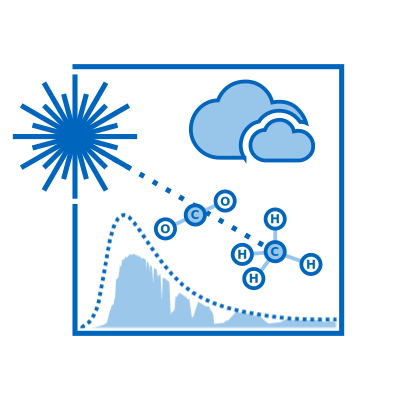
\includegraphics[height=20mm]{template/logos/esm-logo-square.png}
    }{}

\end{titlepage}

\input{template/disclaimer}
\addcontentsline{toc}{chapter}{Acknowledgments}
\thispagestyle{empty}

\vspace*{20mm}

\begin{center}
    {\usekomafont{sectioning}\usekomafont{section} Acknowledgments}
\end{center}

First and foremost, I would like to express my deepest gratitude to my advisor, Moritz Makowski, and professor and supervisor, Prof. Dr. Jia Chen, for their guidance and encouragement.
Their support was incredibly valuable when the challenges at hand seemed almost impossible to overcome.
I am grateful for being entrusted with this novel and challenging idea and for the opportunity to independently research this project.
I do not take this opportunity for granted and am thankful for it.

I also extend my thanks to my friends.
I could not have wished for better ones in my life.
Whenever I faced uncertainties, my friends were my first point of contact.

Lastly, I offer my heartfelt appreciation to my family - my elder brother, my two sisters, and my parents - for their endless love, support, and understanding during tough times.
Although they could not provide much assistance on educational topics throughout my life, I know they would have helped if they could.
They always believed in me, even when I did not believe in myself.
Especially to my parents, I acknowledge how much you have sacrificed to make this education possible and will forever be grateful.
Without my family, this accomplishment would not have been possible.

\vspace{10mm}

\cleardoublepage{}

\chapter{\abstractname}

Dolor aliqua eu labore laboris pariatur velit est est aliquip dolore aliquip minim et. Enim labore adipisicing aliqua anim Lorem. Ex dolor exercitation id cillum consequat laboris. Occaecat id id aute minim sit qui dolore irure pariatur. Enim mollit reprehenderit veniam sunt reprehenderit est aute Lorem dolor veniam.

Laboris ad aliqua fugiat mollit sunt veniam esse cillum excepteur esse do ea veniam. Est ut aliqua culpa ad culpa. Cupidatat ullamco dolore pariatur proident esse minim voluptate dolor ad aliqua incididunt incididunt consequat do. In dolor incididunt in dolore laborum nulla eu nulla dolor fugiat dolore eu.

\clearpage

\glsnogroupskiptrue
\printnoidxglossaries

\clearpage

\microtypesetup{protrusion=false}
\tableofcontents{}
\microtypesetup{protrusion=true}

\mainmatter{}

% !TeX root = ../main.tex
% Add the above to each chapter to make compiling the PDF easier in some editors.

\chapter{Introduction}\label{chapter:introduction}

Global warming poses a significant challenge to our planet and is primarily caused by anthropogenic \gls{GHG} emissions \parencite{IPCC_AR6}.
As a result, climate mitigation has become increasingly important to address this pressing issue.
Emission inventories play an essential role in this effort.
These are collections of emission data of pollutants or \gls{GHG}s released into the atmosphere over a specified period within a defined geographic area.
They serve as foundational tools for environmental management, play a pivotal role in policy formulation, and are essential for compliance with international agreements on climate change mitigation.
Emission inventories are constructed using various techniques, including the bottom-up and downscaling approaches.

The bottom-up approach collects detailed activity data for each emission source, such as fuel consumption rates or industrial production volumes.
Emission factors, representing the average emissions per unit of activity, are then multiplied by these data, resulting in an estimate of the total emissions from that source.
This method enables sectoral analysis, allowing for the identification of crucial emission contributors.

Methods relying on downscaling through spatial proxies, such as those used by the Netherlands Organisation for Applied Scientific Research (TNO) \parencite{TNO_HighRes15, TNO_HighRes18}, start from national-level emission data and disaggregate it to finer spatial scales.
Spatial proxies, such as population density, land use patterns, or road networks, are used to allocate emissions geographically \parencite{SpatialProxies}.

While emission inventories offer detailed estimates, they can be inaccurate due to incomplete data, outdated emission factors, the exclusion of unknown or hidden emission sources, and inaccurate spatial proxy maps \parencite{InventoryUncertainties}.
These limitations underscore the need for inversion techniques, also called top-down approaches.
Top-down approaches promise to close the gap between the actual emissions and those captured by the emission inventories, thus enhancing their comprehensiveness.

Top-down approaches using atmospheric concentration measurements are based on solving ill-posed inverse problems, a widely studied research field.
These approaches formulate the emission estimation problem as an inverse problem, where \gls{GHG} concentrations measured at ground-based or satellite stations are used to infer the underlying emission flux fields based on atmospheric transport.
Examples of sensor networks that perform such measurements include MUCCnet \parencite{MUCCnet} and BEACO\textsubscript{2}N \parencite{BEACON2N}, among others.

From these measurements, top-down approaches reconstruct the emission field by applying inversion techniques.
One such technique is Bayesian inversion, which updates prior knowledge about emissions using a likelihood function derived from measurement data.
Prior knowledge refers to information about emissions before incorporating new measurement data.
However, these methods rely heavily on priors and accurate knowledge about their uncertainties, i.e., assumptions about the emission fluxes, which can introduce bias when information is incomplete or incorrect.

There are many approaches that overcome this limitation of introduced bias, such as geostatistical approaches \parencite{Geostatical}, with recent studies exploring sparse reconstruction techniques \parencite{UrbanSparseReconstruction}. % could add some more here (see Zanger paper)
Sparse reconstruction methods assume that emissions are spatially sparse (i.e., only a few significant sources contribute significantly to the total emissions) and use optimization techniques to recover the emission field from a limited set of measurements.
\textcite{UrbanSparseReconstruction} demonstrated that compressed sensing approaches can be practical for reconstructing \gls{GHG} emissions in urban environments, especially when combined with domain transformations, such as \gls{DWT} \parencite{Wavelets} or \gls{DCT} \parencite{DCT}.

Ill-posed inverse problems arise in many other research fields, including medical imaging.
Significant advancements have been made in this field through machine learning-based compressed sensing techniques \parencite{ReviewCSUsingAI}.
This thesis takes inspiration from these developments and, with advancements in machine learning-based compressed sensing, investigates the applicability of one such approach based on generative models in urban \gls{GHG} emission flux estimation.
The code developed for this research, as well as the model weights, are publicly available on GitHub\footnote{\href{https://github.com/tum-esm/inventory-embeddings}{github.com/tum-esm/inventory-embeddings}}.

% !TeX root = ../main.tex
% Add the above to each chapter to make compiling the PDF easier in some editors.

\chapter{Related Work}\label{chapter:related_work}

\section{Emission Inventories}
Emission inventories are a collection of emission data of pollutants or greenhouse gases (GHGs) released into the atmosphere over a specified period within a defined geographic area.
They serve as foundational tools for environmental management, play a pivotal role in policy formulation, and are crucial for compliance with international agreements on climate change mitigation.
Typically, these inventories are constructed using bottom-up methodologies.
These methods combine individual sources as emissions, providing a comprehensive overview.

The bottom-up approach collects detailed activity data for each emission source, such as fuel consumption rates or industrial production volumes.
Emission factors, representing the average emissions per unit of activity, are then multiplied with these data, resulting in an estimate of the total emissions of that source.
This method makes sectoral analysis possible, thus enabling the identification of crucial emission contributors.

While emission inventories offer detailed estimates, they can be inaccurate due to incomplete data, outdated emission factors, and the exclusion of unknown or hidden emission sources.
These limitations highlight the need for top-down approaches, which use atmospheric measurements to reconstruct emission sources.
Top-down approaches hold the promise of identifying potentially overlooked emitters, enhancing the comprehensiveness of emission inventories.
% Emission inventories are essential tools for monitoring anthropogenic GHG emissions.
% They provide spatially and temporally resolved estimates of emissions based on activity data (e.g., fuel consumption, industrial processes) and emission factors.
% Inventories like the CAMS (Copernicus Atmosphere Monitoring Service) and TNO datasets provide detailed emission fields across Europe with varying spatial resolutions [CAMS 2020; TNO 2020].
% These inventories are typically used for bottom-up estimates, where emissions are computed by aggregating activity data from individual sectors, such as transportation, residential heating, and industry.


% Emission inventories are a estimation of emission fields
% They serve two main purposes \parencite{CAMS-REG-v4}.
% The first purpose is to 
% Questions:
% \begin{enumerate}
%     \item what are the purpose of emission inventories
%     \item what are Emission Inventories
%     \item How are Emission Inventories generated
%     \item what are the problems with bottom-up approaches for GHG emissions? 
%     \subitem may miss
%     \item what are typical approaches to top-down?
%     \item what are the challenges in top-down approaches?
% \end{enumerate}
% Then go over to Benjis work who has shown that 
% For this work, same assumptions as in Benjis work hold, i.e. background GHG emissions are ignored.

% Bottom-up approaches estimate emission fluxes by multiplying emission sources with their activity \parencite{BU-vs-TD} (also cite inventories).
% In contrast, top-down approaches start from measurements of GHG conecntrations and invert the transport of molecules to find the sources from which they emitted.
% One example for a measurement network is MUCCnet \parencite{MUCCnet}.
% Bottom-up approaches can miss emitters due to unknown datas whereas top-down approaches can be able to capture unknown emitters with measurements.
% Furthermore, 
% Bottom-up and top-down approaches show gaps in their esimtations which can largely be explained by temporal variability \parencite{BU-vs-TD}.

% There are essentially two approaches to estimating emissions.
% The first approach starts from the and is called bottom-up approach.
% The second approach starts from measurements and aims at inverting the atmospheric transport of molecules to determine the sources.

% \begin{enumerate}
%     \item 
% \end{enumerate}

\section{Atmospheric Inversion}
Top-down approaches formulate the emission estimation problem as an inverse problem, where GHG concentrations measured at ground-based or satellite stations are used to infer the underlying emission fields.
An example of a sensor network doing such measurements is the MUCCnet sensor network.
From these measurements, top-down approaches reconstruct the emission field by applying inversion techniques. 

One such technique is Bayesian inversion.
Bayesian inversion is a technique that updates prior knowledge about emissions using a likelihood function derived from measurement data [Rodgers, 2000; Ganesan et al., 2014].
Prior knowledge refers to information we have about emissions before we incorporate the new measurement data.
However, these methods rely heavily on accurate priors, which can introduce bias when incomplete or incorrect prior information.
In urban areas, where emissions can vary significantly in space and time, such methods may need prior assumptions to provide accurate results.

Recent studies have explored sparse reconstruction techniques, overcoming the above limitations.
These methods assume that emissions are spatially sparse (i.e., only a few significant sources contribute significantly to the total emissions) and use optimization techniques to recover the emission field from a limited set of measurements.
Works by Benisch et al. (2020) and Turner et al. (2016) demonstrated that compressed sensing approaches can be practical for reconstructing urban GHG emissions, especially when combined with sparse priors or transforms, such as wavelets or discrete cosine transforms (DCT).
% How do top down approaches work?
% What is the inverse problem?
% Benji deonstrated use of compressed sensing.
% Formulate the problem formulation for this thesis here.
% Meaning, what are the constraints.
% Background GHG emissions.
% Assume linear forward model.

% This inverse problem can be solved using Bayesian inversion.
% Mention l2 norm reconstruction.

\section{Compressed Sensing}
Compressed Sensing (CS) is a mathematical framework that enables the recovery of sparse signals from a reduced number of measurements.
The fundamental assumption behind compressed sensing is that the signal of interest is either sparse or compressible in some domain, meaning that most of its components are zero or near zero.
This property allows for the accurate reconstruction of signals even when the number of measurements is significantly smaller than the number of unknowns.

The standard compressed sensing formulation in the context of urban GHG emission estimation is as follows:
\begin{equation}
    y = A x + \epsilon
\end{equation}
where $y \in R$ represents the vector of measurements (e.g., atmospheric GHG concentrations), $A \in R^{m \times n}$ is the sensing matrix that models the relationship between the measurements and the emissions, $x \in R^n$ is the unknown signal (i.e., the emission field), and $\epsilon$ is the noise term, capturing errors or uncertainties in the measurement process.
The sensing matrix $A$ represents the atmospheric transport of molecules and is derived from atmospheric transport models, such as STILT.
Due to a lack of measurements compared to the number of unknowns, this problem is ill-posed.
In urban settings, where emissions are typically sparse, originating from a few dominant sources such as industrial facilities or traffic hubs, compressed sensing provides a natural framework for recovering the emission field from a limited set of observations.

There are many sparse reconstruction algorithms.
One of the most commonly used ones is the Lasso algorithm, which solves the inverse problem by enforcing sparsity through L1-norm regularization.
Another prominent approach is Basis Pursuit (BP), which directly seeks the sparsest solution, and its variant Basis Pursuit with Denoising (BPDN),  which extends the model to handle noisy measurements.
These methods are crucial in emission estimation, where high-dimensional emission fields need to be recovered from a small number of measurements taken by atmospheric sensors.

The Lasso (Least Absolute Shrinkage and Selection Operator) algorithm is a widely used method in compressed sensing due to its ability to enforce sparsity in the solution.
It achieves this by solving the following optimization problem:
\begin{equation}
    \min{\left( \norm{Ax -y }_2^2 + \alpha\norm{x}_1 \right)}
\end{equation}

In this formulation, $\norm{Ax -y }_2^2$ is the least-squares term that measures the difference between the observed measurements $y$ and the predicted measurements $Ax$.
In contrast, the L1-norm $\norm{x}_1$ promotes sparsity.
The parameter $\alpha$ controls the trade-off between the fit's accuracy and the solution's sparsity.
A larger $\alpha$ results in a sparser solution, whereas a smaller $\alpha$ allows for a closer fit to the observed data.
A smaller $\alpha$ may thus introduce non-zero components in $x$, leading to less sparsity.

Basis Pursuit (BP) is another widely adopted algorithm for sparse reconstruction, particularly when the target is to find the sparsest possible solution that satisfies the measurement constraints $y = Ax$ exactly.
Basis pursuit solves the following optimization problem:
\begin{equation}
    \min \norm{x}_1 \quad \text{subject to} \quad  Ax = y
\end{equation}

Here, the objective is to minimize the L1-norm of the signal with the constraint of matching the predicted measurements $A x$ with the observed measurements $y$ exactly.
In contrast to Lasso, basis pursuit does not include a regularization term and instead focuses solely on finding the sparsest solution that satisfies the measurement equation.

Basis pursuit is ideal when the measurement process is noiseless, and the sensing matrix $A$ satisfies the Restricted Isometry Property (RIP), ensuring that different sparse signals remain distinguishable.
However, in real-world applications, such as atmospheric GHG monitoring, measurements are rarely noise-free, and enforcing $Ax = y$ can lead to inaccurate reconstructions when noise is present.

To address the limitations of basis pursuit in noisy environments, Basis Pursuit with Denoising (BPDN) introduces a tolerance for noise in the measurement process.
BPDN modifies the original basis pursuit problem by allowing deviations from the exact measurement equation:
\begin{equation}
 \min \norm{x}_1 \quad \text{subject to} \quad  Ax -y \le \delta
\end{equation}

In this formulation, $\delta$ represents the allowable level of noise or error in the measurements.
Again, the L1-norm is minimized to promote sparsity in the signal, while the L2-norm ensures that the predicted measurements are close to the observed measurements within a defined noise threshold.
The parameter $\delta$ allows BPDN to flexibly handle noisy data, making it more suitable for real-world scenarios, such as urban GHG emission estimation, where measurement noise is inevitable due to sensor inaccuracies and atmospheric variability.

Basis Pursuit with Denoising strikes a balance between sparsity and measurement accuracy. It is beneficial when the sensing matrix $A$ does not fully satisfy RIP, or the measurement process involves significant noise.
By allowing for a controlled level of error, BPDN can recover the sparse emission field without being overly sensitive to noise.
This means that BPDN can tolerate a certain amount of noise in the measurements, ensuring robust solutions.

I should probably add the advantages of Lasso vs BPDN and vice versa.
They can be shown to be quivalent for some $\alpha$, but this also means that Lasso requires tuning of $\alpha$.
However, Lasso is computationally more efficient.
In cases where the computational complexity is not a problem, this thesis will make use of BPDN.

I should also probably put some notes on transformations which makes signal more sparse.

\section{Generative Models for Compressed Sensing}
As mentioned, compressed sensing traditionally assumes that the underlying signals are sparse on some basis.
However, this assumption may only hold in some applications.
For instance, in urban emissions scenarios, while large point sources are often known or can be well-estimated, diffuse or area sources result in emission fields that are less sparse.
This lack of sparsity challenges the effectiveness of conventional compressed sensing techniques, potentially leading to reconstruction failures.

Generative models offer a promising alternative by relaxing the strict sparsity constraint.
These models learn complex representations directly from data, circumventing the need for pre-specified sparse bases.
Recent advancements in fields such as medical imaging have successfully applied generative models to solve compressed sensing problems (cite). %\parencite{jalal2021robust}).

In this thesis, we focus on the pioneering work by Bora et al. (cite), a framework that leverages generative models to improve upon classical compressed sensing techniques.
Their approach demonstrates that using neural networks trained to model the distribution of the underlying data can significantly enhance the performance of compressed sensing.

\subsection{Generative Models}

Bora et al.'s framework primarily involves generative adversarial network (GAN) type models, including Variational Autoencoders (VAEs) and Generative Adversarial Networks (GANs).
Both VAEs and GANs generate samples from lower-dimensional noise, transforming a latent variable $z \in \mathbb{R}^d$ into a data sample $x \in \mathbb{R}^n$ through a generator function $G: \mathbb{R}^d \to \mathbb{R}^n$.

Variational Autoencoders (VAEs) are probabilistic models that encode input data into a latent space and then decode it back to the original space.
They optimize a variational lower bound on the data likelihood, effectively learning a smooth latent space that captures the data distribution.

Generative Adversarial Networks (GANs) consist of two neural networks, a generator $G$ and a discriminator $D$, trained in a minimax game.
The generator tries to produce data that is indistinguishable from real data, while the discriminator attempts to differentiate between real and generated data.
GANs are known for generating high-quality samples but can be challenging to train due to instability in the adversarial objectives.

While GANs often show superior quality in sample generation across various domains, their training instability makes them less suitable for some applications.
Therefore, this thesis chooses VAEs as the appropriate type of generative model due to their stability and structured latent space.

Besides Bora et al. work there are many different approaches (cite the overview).
For example, work using score-based or diffusion models (cite) in the context of medical imaging (cite).
Additionally, normalizing flows (cite) also show promising reults (cite).
But since the goal of this thesis is not to compare individual ML based compressed sensing approaches, the focus lies on Bora et al. work.

\subsection{The Range of a Generator}

The range of a generator $G$ refers to the set of all possible outputs $G(z)$ as $z$ varies over the latent space $\mathbb{R}^d$.
This range represents the subset of the signal space $\mathbb{R}^n$ that the generative model can produce.
In the context of compressed sensing, the reconstruction is constrained to lie within this range, which underscores the importance of the generative model accurately capturing the true data distribution.

\subsection{Compressed Sensing Framework}

Bora et al.'s approach integrates generative models into the compressed sensing reconstruction process.
Given a linear measurement model:
\begin{equation}
 y = A x + \epsilon
\end{equation}
where $A \in \mathbb{R}^{m \times n}$ is the sensing matrix, $x \in \mathbb{R}^n$ is the unknown signal (e.g., an emission field), $y \in \mathbb{R}^m$ represents the measurements, and $\epsilon$ denotes noise, the goal is to recover $x$ from $y$.

The key idea is to leverage a pre-trained generative model $G$ as a prior for $x$.
In contrast to Bayesian inversion, which heavily relies on a predefined prior, which can be a significant limitation if the prior does not accurately reflect the actual spatial distribution of emissions, the prior is more robust.
A generative model would avoid this by learning the prior directly from the data.
The reconstruction problem is formulated as an optimization over the latent space:

\begin{equation}
 \min_{z}{\left( \norm{A G(z) - y}_2^2 + \gls{gamma} R(z) \right)}
\end{equation}
Here, $R(z)$ is a regularization term that encourages desirable properties in the solution, and $\gls{gamma}$ controls the strength of the regularization.
For instance, in the case of $z$ being Gaussian distributed, the regularization $R(z) = \norm{z}_2^2$ can be used, similar to Ridge regression.
The generative model $G$ represents the range of possible signals, and the optimization seeks the latent vector $z$ that, when passed through $G$, produces a signal that matches the measurements $y$ as closely as possible.

Since $G$ is differentiable with respect to $z$, gradient-based optimization methods can be employed to solve the problem.
The optimization seeks the latent vector $z^{\star}$ such that $G(z^{\star})$ best explains the measurements $y$.

\begin{figure}[h!]
    \centering
    \includegraphics[width=0.75\textwidth]{figures/02_related_work/latent_variable_optimization/build/latent_variable_optimization.pdf}
    \caption{Bora et al paper}
    \label{fig:gen_solver}
\end{figure}

One limitation of Bora et al.'s method is that the reconstructed signal $G(z^{\star})$ is confined strictly to the range of $G$.
This constraint may be too restrictive if $G$ does not perfectly capture the data distribution, leading to reconstruction errors.

Dhar et al. (cite) proposed an extension that allows for sparse deviations from the generator's output to address this issue.
The modified optimization problem introduces an additional variable $s \in \mathbb{R}^n$ representing a sparse offset:

\begin{equation}
 \min_{z, s}{\left(\norm{s}_1 + \gls{lambda} \norm{A \left( G(z) + s \right) - y}_2^2 \right)}
    \label{eq:sparse_deviation}
\end{equation}
where $\norm{s}_1$ promotes sparsity in the offset $s$ and the parameter $\lambda$ balances the sparsity of $s$ with the fit to the measurements $y$.

The reconstructed signal is then given by $\hat{x} = G(z^\star) + s^\star$, where $z^\star$ and $s^\star$ are the solutions to the optimization problem in Equation \ref{eq:sparse_deviation}.

This extension allows the reconstruction to deviate slightly from the generator's range, accommodating components of the signal not captured by $G$, while maintaining overall consistency with the measurements and promoting sparsity in the deviations.

\section{Contributions}
In this work we make the following two assumptions:
\begin{enumerate}
    \item background emissions are known
    \item large emitters are accurately estimated
\end{enumerate}

The point of this work is not to investigate whether compressed sensing theory can be applied in the context of 
This has been investigated by prior work, like Benjis.
The point of this thesis is to investigate whether generative models can be applied.

Is the model able to generalize beyond the trianing data?
Is the model able to reconstruct emitters that are not covered in the emission inventories? 
What is a good dimension for the lower dimensional space?

Mention the rough constributions of this work:
\begin{enumerate}
    \item trained VAE for emission inventories of European cities
    \item demonstrated the applicability of generative models in the context of inverse models for top-down approaches
\end{enumerate}


\section{Contributions}
In this work we make the following two assumptions:
\begin{enumerate}
    \item background emissions are known
    \item large emitters are accurately estimated
\end{enumerate}

The point of this work is not to investigate whether compressed sensing theory can be applied in the context of 
This has been investigated by prior work, like Benjis.
The point of this thesis is to investigate whether generative models can be applied.

Is the model able to generalize beyond the trianing data?
Is the model able to reconstruct emitters that are not covered in the emission inventories? 
What is a good dimension for the lower dimensional space?

Mention the rough constributions of this work:
\begin{enumerate}
    \item trained VAE for emission inventories of European cities
    \item demonstrated the applicability of generative models in the context of inverse models for top-down approaches
\end{enumerate}

% !TeX root = ../main.tex
% Add the above to each chapter to make compiling the PDF easier in some editors.

\chapter{Dataset}\label{chapter:dataset}

This thesis aims to develop a compressed sensing framework that leverages the strengths of deep generative models.
Methods proposed by \textcite{CSUsingAI} have demonstrated superior reconstructions with fewer measurements than classical compressed sensing techniques.
Consequently, this thesis focuses on reconstructing ill-posed problems with many unknowns.

Datasets with high spatial resolution inventories are required to facilitate this.
Datasets like CAMS-REG-v4 \parencite{CAMS} provide \gls{GHG} emissions at a resolution of $0.1^{\circ}$ latitude by $0.05^{\circ}$ longitude, which corresponds to approximately $5$ by $5$ kilometers over central Europe.
This resolution is relatively low.
For example, a city spanning a $30 \unit{km}$ by $30 \unit{km}$ area would be divided into a spatial grid of $6$ by $6$ cells.
Therefore, this thesis utilizes the high-resolution inventories TNO-GHGco-v1.1 for $2015$ emissions \parencite{TNO_HighRes15} and TNO-GHGco-v4 for $2018$ emissions \parencite{TNO_HighRes18}.
These inventories provide emissions at spatial resolution of ${{}^{1}\!/\!{}_{120}}^\circ$ latitude by ${{}^{1}\!/\!{}_{60}}^\circ$ longitude, or approximately $1 \unit{km}$ by $1 \unit{km}$.
This high spatial resolution allows for extracting detailed emission fields in urban environments.
The inventories include \gls{GHG} emissions for each GNFR sector, with the road sector (sector F) further divided into four subsectors, for each coordinate in a defined European grid.
This results in $15$ emission values per gas per cell.

In this thesis, only $\text{CO}_2$ emissions from fossil fuels (ff) are considered.
However, the approaches presented can be directly applied to all \gls{GHG} sources.
Furthermore, as point sources are assumed to be known, only diffuse or area sources are extracted from the inventories.
Finally, it has to be noted that the following approximation is made: one grid cell has the spatial dimension of exactly $1 \unit{km}$ by $1 \unit{km}$.
While this may result in improper scaling of values for many cities, the final results remain unaffected due to the invariance of the inverse problem to scale.

\section{Urban Emission Fields}
Urban environments differ from non-urban environments in terms of their emissions.
For instance, urban environments often have a city center that generates a large portion of emissions, as can be seen in Munich in Figure \ref{fig:munich_emissions}.
\begin{figure}
    \centering
    \begin{subfigure}{0.32\textwidth}
        \centering
        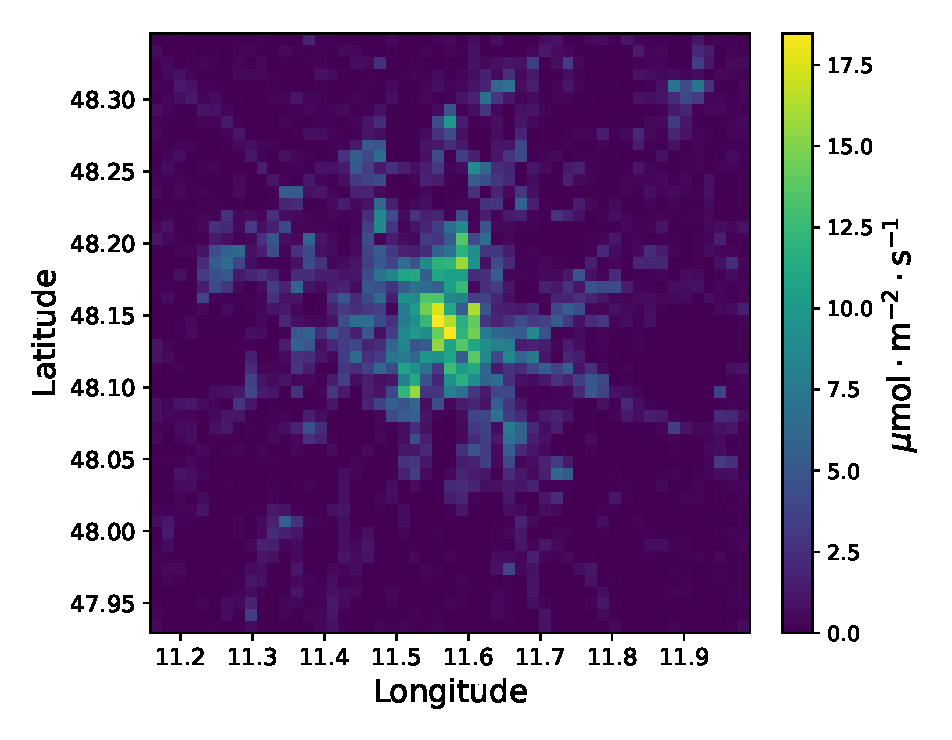
\includegraphics[width=\linewidth]{figures/03_dataset/munich/munich_2015_total_emissions.eps}
        \caption{Total Emission Fluxes}
    \end{subfigure}
    \begin{subfigure}{0.32\textwidth}
        \centering
        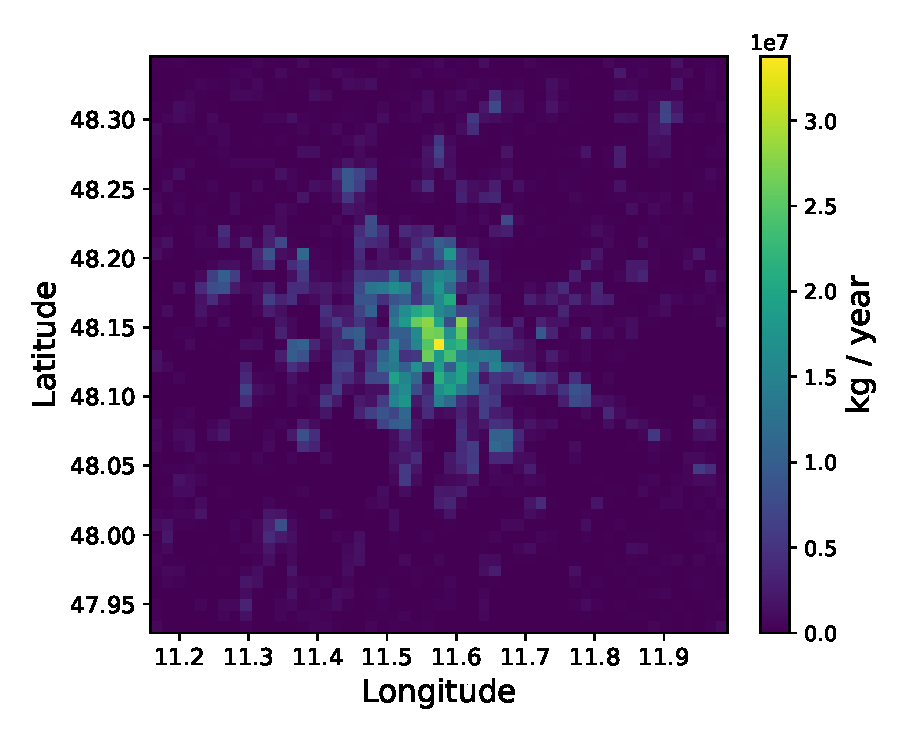
\includegraphics[width=\linewidth]{figures/03_dataset/munich/munich_2015_sector_c.eps}
        \caption{GNFR Sector C}
    \end{subfigure}
    \begin{subfigure}{0.32\textwidth}
        \centering
        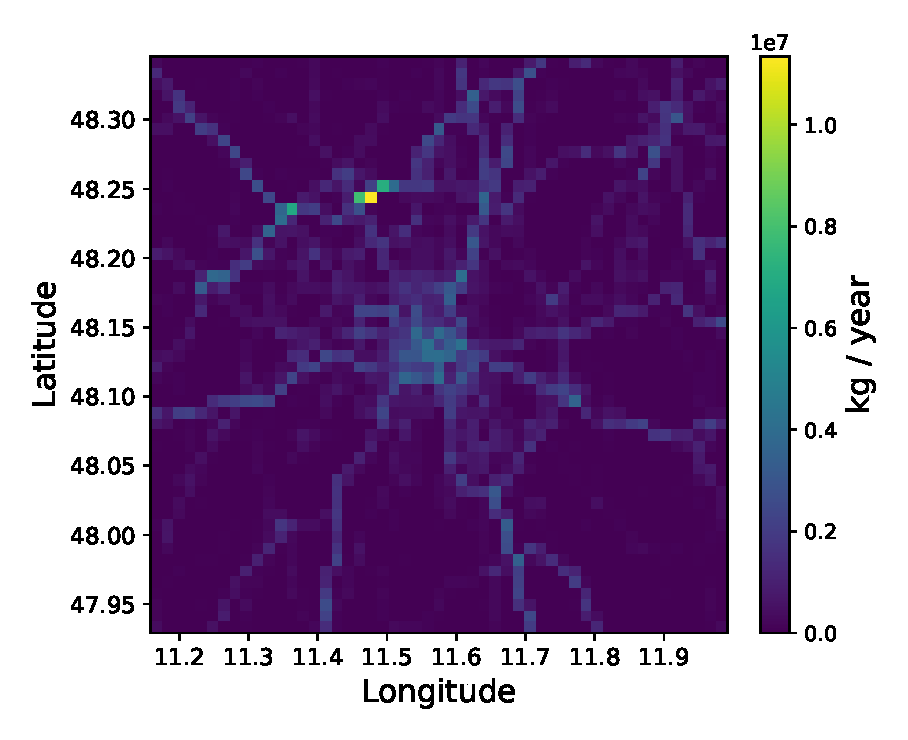
\includegraphics[width=\linewidth]{figures/03_dataset/munich/munich_2015_sector_f1.eps}
        \caption{GNFR Sector F1}
    \end{subfigure}
    \caption{$\text{CO}_2$ (ff) Emission Fluxes from Area Sources in Munich in 2015 \parencite{TNO_HighRes15}}
    \label{fig:munich_emissions}
\end{figure}
Therefore, as this thesis focuses on urban environments, they have to be filtered from the TNO-GHGco datasets.
For this, several cities are selected from a public database by OpenDatasoft \parencite{OpenDataSoft}.
Cities are filtered according to their population size.
For this thesis, we define a population threshold of $100,000$.
Any cities with a population greater than $100,000$ are selected for the dataset.

The coordinates of the filtered cities are then used to extract emission fields.
From the inventories, $51$ by $51$ grid cells around the city center are extracted.
This corresponds to a dimension of approximately $51 \unit{km}$ by $51 \unit{km}$. 
While most cities are not even close to this size, this allows for later cropping of the fields to a desired size.
For this thesis, emission fields have a final size of $32$ by $32$.

Some cities may be too close to each other, resulting in data leakage to test and validation sets.
Thus, cities are filtered if they are too close to other cities.
The following algorithm guarantees that no cities in the dataset overlap.

\begin{quotation}
First, an empty list of extracted lists is initialized.
Then, for each city, the latitude and longitude distances to all extracted cities are calculated.
In the next step, the algorithm determines which cities fall within a defined distance threshold from the current city.
If no cities are found within this threshold, the current city is added to the list, and the algorithm moves on to the next city.
However, if overlapping cities are identified within the threshold, the population size of the current city is compared to those of the overlapping cities.
If the current city has a larger population than all of the overlapping cities, these cities are removed, and the current city is added to the list.
If the current city does not have a larger population, it is ignored, and the algorithm continues with the next city.
\end{quotation}

This extraction results in $106$ city emission fields per year, $2015$, and $2018$.
However, we identified Bratislava as an outlier for this dataset due to its high \gls{SSIM} with a $0$ emission field.
Therefore, we exclude Bratislava from the dataset, thus reducing the number of cities to $105$.

This limited number of extracted emission fields is insufficient to train a generative model.
Thus, temporal scaling factors from \parencite{ScalingFactors} are useful for artificially generating more samples.
Scaling factors are applied to individual GNFR sectors.
This results in $24 \cdot 7 \cdot 12 = 2016$ samples per city per year.
The resulting combined dataset size is then $105 \cdot 2 \cdot 2016 = 423,360$ individual emission fields with size $51$ by $51$.
Scaling factors are applied at sampling time to reduce memory overhead, thus only keeping the original data in memory.

\section{Dataset Split}
The emission fields are divided into training, validation, and test sets.
The test set comprises $t$ percent of the data and is used exclusively for experiments and evaluations; the model does not encounter this data during training.
The validation set makes up $v$ percent of the data and is used during training to assess the model's generalization capabilities.
The remaining data, i.e., $1-v-t$ percent, is allocated to the training set for updating the model's weights.

A random split could result in unrepresentative subsets since emission fields of cities may vary significantly in their mean emissions.
For example, if the validation set contains cities with higher mean emissions, the \gls{MSE} during validation would be higher due to \gls{MSE}'s sensitivity to scale.
Therefore, it is essential to distribute cities equally across the training, validation, and test sets concerning their mean emissions to best assess generalization abilities.
Additionally, data from individual cities should not be split across different datasets to prevent data leakage.
For instance, Berlin's data from $2015$ should not be in the test set if its $2018$ data is in the training set.

The following algorithm fulfills both requirements from above while producing a reproducible split:

\begin{quotation}
First, the algorithm groups the emission fields according to their city name.
The emission fields are then sorted alphabetically according to the above names.
In the second step, the algorithm sorts the emission fields by their mean emissions in descending order.
Finally, it splits the dataset using equidistant indices to produce two datasets.
\end{quotation}

This algorithm is then used to assign $t$ percent of the data to the test set.
Then, from the remaining $1 - t$ percent, $\frac{v}{1 - t}$ percent is assigned to the validation set.
The rest is allocated to the training set.

\section{Data Augmentation}
To enhance the generalization capabilities of the model, we apply common image augmentation \parencite{ImageAugmentation} to the emission fields in the training dataset.
The augmentation methods applied include random cropping, flipping, and rotation.
To introduce variability in spatial positioning, emission fields are randomly cropped to a spatial dimension of $32$ by $32$.
Additionally, with a probability of $0.5$, the emission fields undergo horizontal or vertical flipping.
Similarly, with a probability of $0.5$, they are rotated by $90$ degrees.
These techniques result in eight possible transformations for each emission field, including the original unaltered version.

An example of this augmentation process is illustrated in Figure \ref{fig:nuernberg_emissions}.
The figure shows the original and transformed emission fields for the Nuremberg area sources, highlighting how the summed emissions are altered through the applied transformations.

\begin{figure}[h!]
    \centering
    \begin{subfigure}{0.4\textwidth}
        \centering
        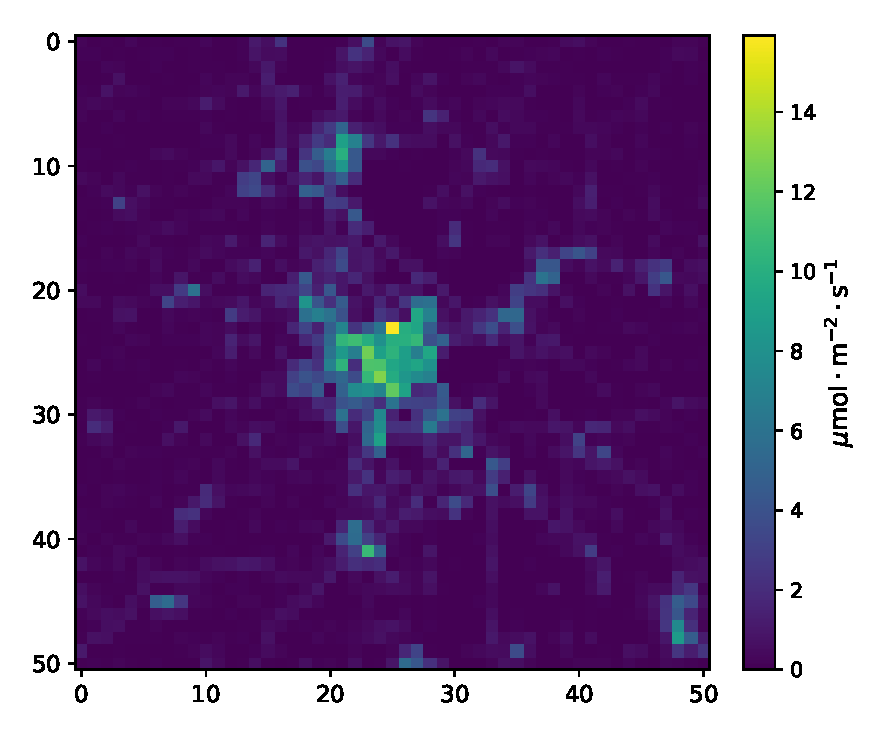
\includegraphics[width=\linewidth]{figures/03_dataset/nuernberg/nuernberg.eps}
        \caption{Original}
    \end{subfigure}
    \begin{subfigure}{0.4\textwidth}
        \centering
        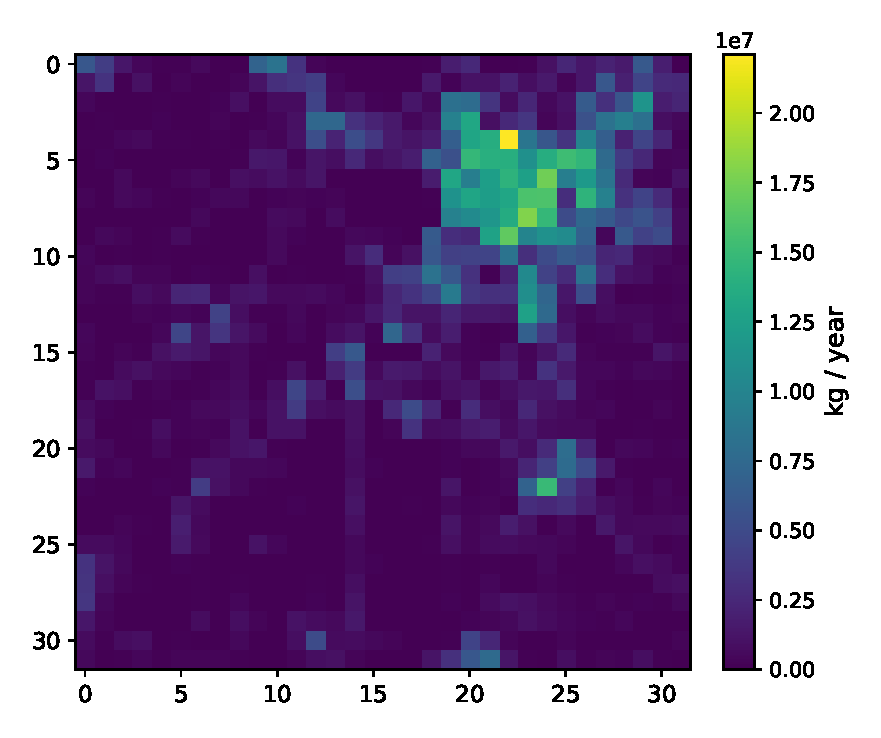
\includegraphics[width=\linewidth]{figures/03_dataset/nuernberg/nuernberg_transformed.eps}
        \caption{Transformed}
    \end{subfigure}
    \caption{Total $\text{CO}_2$ (ff) Emission Fluxes from Area Sources in Nuremberg in 2015 \parencite{TNO_HighRes15}}
    \label{fig:nuernberg_emissions}
\end{figure}

It is important to note that these transformations are not applied to the validation and test emission fields, except for a center crop to match the expected input dimensions.

\section{Scaling}
Scaling plays an important role in machine learning.
Large-scale data can make training converge slowly and become unstable \parencite{DataScaling}.
A common technique for scaling values is min-max scaling \parencite{MinMaxScaling}.
However, min-max scaling is sensitive to outliers and thus not ideal for emission inventories where the range of emissions within a city can vary greatly.
Instead, robust scaling can be applied.
To determine a good scaling factor, the $95$th percentile of values is determined for each city in the training set.
The inverse of the average is then used as the scaling factor.
The resulting scaling factor is thus $\frac{1}{2.5 * 10^6}$ after rounding.
All experiments are, without loss of generality, performed on the scaled data.

\section{Case Studies}
In addition to the test data used for model performance evaluation, three cities are selected for detailed case studies.
The cities are Munich, Zurich, and Paris.
These cities are chosen based on the ICOS Cities PAUL project \parencite{Icos} and represent a range of city sizes, from small to medium and large.
In order to ensure unbiased results, these cities are excluded from the dataset prior to splitting, reducing the total number of cities available for training from $105$ to $102$.
These cities allow closer inspection of the outputs of different algorithms.

% !TeX root = ../main.tex
% Add the above to each chapter to make compiling the PDF easier in some editors.

\chapter{Variational Autoencoder}\label{chapter:vae}

Some text about generative models and variational autoencoder \parencite{VAE} in its original form being the chosen one.

\section{Architecture Search}
Searching for optimal hyperparamaters is a challenging task with many different approaches \parencite{HyperParameters}.
In particular, designing a good architecture takes a lot of trial and error.
Thus, different architectures are explored to determine a suitable one.
For this, first a basline architecture is established.
Then, different variations of this architecture are explored and trained.
The architecture of the model with the best performance is then chosen as the model architecture for this thesis.

Each variation is trained with for $20$ epochs on the TNO 2015 data only to decrease the architecture bias during search.
The dataset split is $t=0.15$, $v=0.15$, with the test set not being used at all.
The batch size is $32$.
As optimizer AmsGrad \parencite{AmsGrad} is used with a learning rate of $\dots$.
Gradients are clipped at $0.5$.
% Add any further hyperparameters.

\section{Baseline Architecture}
The baseline architecture is inspired by \parencite{Tightrope}.
This means that the bottleneckl layers have a high width and height.
As the input width and height of the emission fields are $32$ by $32$, the Bottleneck width and height are chosen as $8$ by $8$.
Inspired by \parencite{AllConvolutional} , to reduce the width and height dimensions, instead of using pooling operations, $2$ strided convolutions are used.
The strided convolutions, depicted in Figure, have kernel 2 and stride 2, thus halfing the size.

\begin{figure}[h!]
    \centering
    \begin{minipage}[b]{0.45\textwidth}
        \centering
        \includegraphics[]{figures/model_architecture/build/conv_layer.pdf}
        \caption{Conv Layer}
    \end{minipage}
    \hfill
    \begin{minipage}[b]{0.45\textwidth}
        \centering
        \includegraphics[]{figures/model_architecture/build/deconv_layer.pdf}
        \caption{DeConv Layer}
    \end{minipage}
\end{figure}

The strided convolution layers make use of the LeakyReLu activation function and batch normalization \parencite{BatchNorm}, as a regularization technique.

Vice versa, in the decoder, 2 strided transpose convolutions with the same parameters are used to double the width and height instead of upsampling layers.

In between the strided convolutions residual convolutional layers (ResConv) \parencite{ResNet} are used.
They can be seen in Figure.
\begin{figure}[h!]
    \centering
    \includegraphics[]{figures/model_architecture/build/residual_conv_layer.pdf}
    \caption{ResConv Layer \parencite{ResNet}}
\end{figure}
The ResConv layers make use of two convolutions with kernel 3 and padding 1 to retain the width and height dimensions.
The output activation is ReLu.
In between the two convolutional layers, LeakyReLu is used again.
Again, batchnorm is applied.
\begin{figure}[h!]
    \centering
    \includegraphics[width=\textwidth]{figures/model_architecture/build/baseline_vae_encoder.pdf}
    \caption{Baseline Encoder Architecture (generated with \parencite{NNVisualization})}
\end{figure}
\begin{figure}[h!]
    \centering
    \includegraphics[width=\textwidth]{figures/model_architecture/build/baseline_vae_decoder.pdf}
    \caption{Baseline Decoder Architecture (generated with \parencite{NNVisualization})}
\end{figure}
As can be seen in Figure and Figure, the 2 strided convolutions are located between $2$ layers of ResConv layers each, in the encoder and decoder.
Fully connected layers are used at the end of the encoder and beginning of the decoder to achive a hidden dimension $256$ of the latent space. 
The last ResConv layers does not use batch normalization.
The number of parameters is \dots.

The loss function used is the typical VAE loss with MSE loss as recontruction loss and Elbo \parencite{VAE} \dots .
\begin{equation}
    L(x, \hat{x}) = 1 + 2
\end{equation}
In addition to the loss, at each step the SSIM \parencite{SSIM} is computed as it provides qualitatively better comparison between two emission fields than the MSE as it takes structure into account.

\section{Explored Variations}
The following variations are explored
\begin{enumerate}
    \item conv layers to increase / decrease depth and pooling layers to decrease width/height and upsample layers to increase width/height
    \item upsampling emission fields to $64$ by $64$ and then applying convlutions; in decoder max pooling to downsample $64$ by $64$ to $32$ by $32$
    \item more depth; instead of doubling depth, quadrupling it
    \item 2 conv layers for changing width and height instead of one strided convolution
    \item 3 ResConv layers everywhere
    \item residual layers with identity mappings depicted in Figure based on \parencite{IdentityMappings} instead of ResConv layers from Figure
    \item residual layers with identity mappings with dropout \parencite{Dropout} based on \parencite{WideResNet} (add explanation)
\end{enumerate}

\begin{figure}[h!]
    \centering
    \includegraphics[]{figures/model_architecture/build/residual_conv_with_im_layer.pdf}
    \caption{ResConv Layer With Identity Mappings \parencite{IdentityMappings}}
\end{figure}

In Figure , the validation losses and validation SSIM can be seen from the 20 epoch trianing runs.

\begin{figure}
    \centering
    \begin{subfigure}{0.49\textwidth}
        \centering
        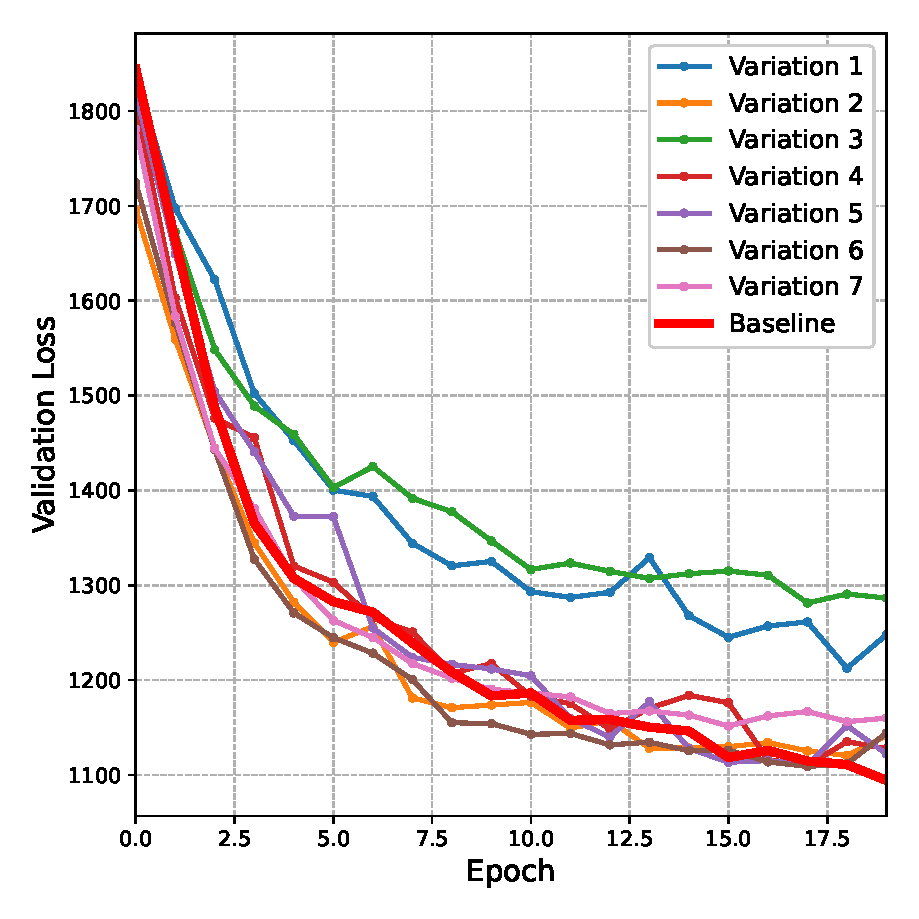
\includegraphics[width=\linewidth]{figures/architecture_search/architecture_search_loss.eps}
        \caption{Validation Loss}
        \label{fig:sub1}
    \end{subfigure}%
    \begin{subfigure}{0.49\textwidth}
        \centering
        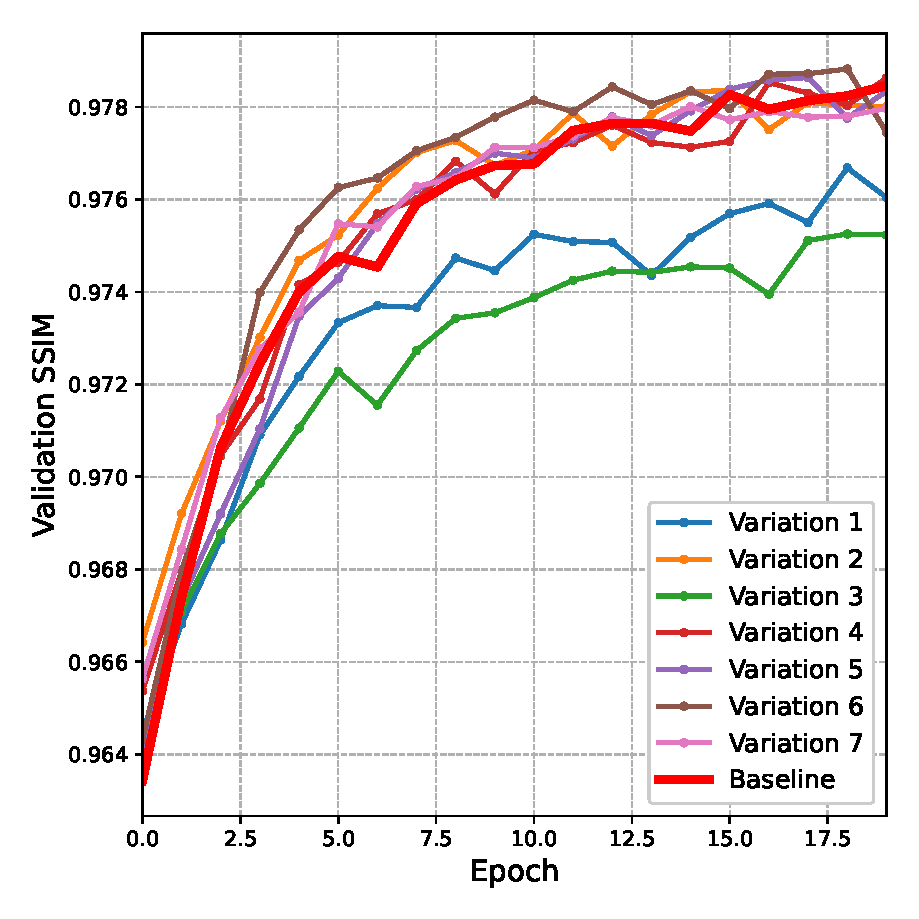
\includegraphics[width=\linewidth]{figures/architecture_search/architecture_search_ssim.eps}
        \caption{Validation SSIM}
        \label{fig:sub2}
    \end{subfigure}
    \caption{Performance of Variations on Validation Data During Training}
    \label{fig:test}
\end{figure}

Add some observations.

\section{Final Architecture}
From the previous subsection, it can be concluded that the baseline architecture performs very well.
The following changes are made to result in the final architecture.
First, the residual layers in Figure  with identity mappings are used.
Furthermore, they are extended with dropout as proposed in \parencite{WideResNet} in the \dots.
Finally, the number of residual layers are increased to $3$.
The encoder and decoder respectively can be seen in Figure and Figure.
\begin{figure}[h!]
    \centering
    \includegraphics[width=\textwidth]{figures/model_architecture/build/final_vae_encoder.pdf}
    \caption{Final Encoder Architecture (generated with \parencite{NNVisualization})}
\end{figure}
\begin{figure}[h!]
    \centering
    \includegraphics[width=\textwidth]{figures/model_architecture/build/final_vae_decoder.pdf}
    \caption{Final Decoder Architecture (generated with \parencite{NNVisualization})}
\end{figure}
The latent dimension $d$ which was kept at $d = 256$ for the "ablation study" is now kept parametrizable.
In fact, for this thesis, different latent dimensions are explored: $d \in \{ 256, 512, 1024, 2048 \}$.
The number of parameters of the model in dependence of $d$ are \dots.

\begin{table}[h]
    \centering
    \begin{tabular}{|c|c|c|}
        \hline
        \textbf{$d$} & \textbf{Encoder Parameters} & \textbf{Decoder Parameters} \\
        \hline
        \hline
        $256$ & 2.2 M & 1.3 M \\
        $512$ & 4.2 M & 2.2 M \\
        $1024$ & 8.1 M & 4.2 M \\
        $2048$ & 16.0 M & 8.1 M \\
        \hline
    \end{tabular}
    \caption{Number of Encoder / Decoder Parameters in Dependence of Latent Dimension $d$}
    \label{tab:num_parameters}
\end{table}

The models are trained on both the TNO 2015 and 2018 data for $100$ epochs.
The dataset split is $t = 0.13$ and $v = 0.15$, resulting in $13$ cities in the test, $15$ cities in the validation, and $74$ cities in the training set.
The exact split can be seen in appendix \dots.
The weights of the model with the highest validation SSIM during the $100$ epochs is stored.
All other relevant hyperparamaters are kept the same as in the the variations subsection.

The training losses, SSIM, and mean MSE can be seen in Figure for each $d$.
(add Figure).
It can be observed that there is overfitting present in the data.
This may be related to samples like London or Berlin in the trianing data that steer the loss, resulting in overfitting to these cities, due to their size of emissions.
The amount of overfitting decreases with an increase in $d$.


\section{Fine-tuning}
Fine-tuning is a popular technique to steer a model to do somthing more specific \cite{FineTuning}.
In the case of this thesis, fine-tuning the trained model to specific cities may make sense to achieve more precise recontruction.
The idea is that a generative model can learn the structure of the city and focus on differences of emissions due to observed data.
Thus, fine-tuning is evaluated in this thesis.
For this, the three for the case studies chosen cities are used.

The idea of fine-tuning the model to specific cities is to move the range $R(G)$ of the generator $G$, i.e. the space of all emission fields generateable by the decoder of the VAE.
For instance, if a model cannot represent an emission field that is to be sensed, it is not able to reconstruct the emission field due to a high representational error.
By fine-tuning the model, the range of the generator is modified such that the emission field to be sensed may either be closer to the range of the generator or even in it.
This is depicted in Figure (make figure here to show the idea).

During fine-tuning, the weights of the original models are updated.
The learning rate is reduced.
In our case, we chose $10^{-x}$ as learning rate.

For fine-tuning, the TNO 2015 data is used.
Later, for evaluation the TNO 2018 is used.

The cities are cropped in the center.
Furthermore, random scaling factors $s \in U(0.5, 1.5)$ are applied to simulate uncertainties in emission inventories.
Additionally, gaussian noise is added to the city emission field.

Models are fine-tuned for $30$ epochs which results in errors close to convergence.


% !TeX root = ../main.tex
% Add the above to each chapter to make compiling the PDF easier in some editors.

\chapter{Compressed Sensing}\label{chapter:compressed_sensing}

\section{Inverse Problems}
To evaluate the generative capbailities in the context of inverse problems, compressed sensing problems are used for evaluation.
The compressed sensing problem is defined using a sensing matrix $A \in R^{m \times 15360}$.
The forward model is then defined as
\begin{equation}
    y = A x + \epsilon
\end{equation}
The signal $x \in R^{15360}$ is derived from an emission inventory $\hat{x} \in R^{32 \times 32 \times 15}$ that is vectorized, i.e. $x = \text{vec}(\hat{x})$.
The Gaussian noise $\epsilon \in R^m$ is sampled from a zero mean Gaussian distribution $N(0, \sigma)$.
The standard deviation of $\sigma \in R$ depends on a paramtrizable signal to noise ratio SNR and the signal power $SP = \frac{1}{m}\sum_{i=1}^m{\left(Ax\right)_i}$ of the measurements.
\begin{equation}
    \sigma = \sqrt{\frac{SP}{SNR}}
\end{equation}

\subsection{Gaussian Measurements}
This compressed sensing problem is based on the paper by Bora et al. as they mention that the performance of generative models can be assesed based on their provided problem statement.
For this, a identically independent distributed matrix $A \in R^{m \times 15000}$ is sampled for each run.
The following inverse problem is then solved using the minimization problem proposed by Bora et al \parencite{CSUsingAI}.

with $x$ being the emission fields $x^*$ in vectorized form.
This inverse problem is equivalnt to taking taking $m$ measurements that is randomly linearly affected by any sector in any cell within the emission field grid.
While this does not correspond to a physical transport model which follows the law of physics, this problem serves as a good proxy for evaluating the generative capbailities in the context of inverse problems of the trained VAE. 
The randomly sampled sensing matrix fulfills the ... properties and thus allows comparision of solvers in ideal scenarios.
This allows assessing the the potential of solvers independent of outside variables.

The evaluation is performed on scaled emission fields.

The resulting pipeline is the following:
\begin{enumerate}
    \item Generate random A
    \item Sample x from test set
    \item Vectorize x
    \item Compute y from forward model
    \item Run reconstruction algorithm (minimization problem)
    \item Unvectorize resulting x dach
    \item Compare x with x dach
\end{enumerate}

The reconstruction algorithm is run for the following number of measurements:
For each of the numbers, the reconstruction is run for each emission field in the test dataset.
A random measurement matrix $A$ is generated and each of the $3$ algorithms solve the same inverse problem.
The temporal transforms are disabled during evaluation which means that for each city only one emission field per year is used.
The evaluation is run 5 times to reduce randomness resulting from random initialization of $z$.

\subsection{Gaussian Plume Model}
Gaussian sensing matrix do not represent the real the emission problem well.
Instead of randomly samples sensing matrices, transport models should be used that indicate the sensitivity of measurements with resepect to physical grid cells based on the transport of molecules in the past.
These transport models are computationally expensive and in generel difficult to estimate on a per city basis.
Thus, we apply the same idea as Benji in his work.
We substitue typical transport models, such as STILT, with a Gaussian plume model.
We want to apply the model to reconstruct total emissions from area sources, i.e. 32 by 32.
The generative models are trained to reconstruct sector-wise.
Thus, we can reconstruct the decomposition into sectors and the sum each sector to achieve reconstruction of total emissions.
This is a more challenging task for the generative model.
If it were directly trained on generating 32 by 32 fields, the results would be much better.

Furthermore, we consider the case of make measurements from the field containing point sources.
Measurements are thus computed as follows:
\begin{equation}
    y = A x + \epsilon
\end{equation}
The emissions can now be decomposed into area and point source fields.
\begin{align}
    y &= A (x_A + x_P) + \epsilon \\
    y &= A x_A + A x_P + \epsilon \\
    y - A x_P &= A x_A + \epsilon \\
    \tilde{y} &= A x_A + \epsilon
\end{align}

\subsection{Gaussian Plume Model 2}

In his paper, Benji reconstructed the emission field without considering the indivudal sectors as contributors.
In this thesis, a full reconstruction is attempted, i.e. all $15$ sectors are reconstructed.
Therefore, the sensing matrix based on the Gaussian plume model must be adapted accordingly.

Consider measurement in the spatial domain, i.e. in the $32$ by $32$ grid.
A measurement would then be affected by the sum of all emitters of each sector.
We denote $x_S = x_A + x_B + \dots x_L$, where $x_i$ corresponds to the emissions of sector $i \in \{A, B, \dots, L\}$, as the sum of all sectors.
Then, the forward sensing model has the following form.
\begin{equation}
    y = A_S x_S + \epsilon
\end{equation}
This can be formulated as follows:
\begin{align}
    y &= A_S (x_A + x_B + \dots + x_L) + \epsilon \\
    y &= A_S x_A + A_S x_B + \dots + A_S x_L + \epsilon \\
\end{align}
Rewriting this as a matrix multiplication yields the following
\begin{equation}
    y = \begin{bmatrix} A_S & A_S & \cdots & A_S \end{bmatrix}\begin{bmatrix} x_A \\ x_B \\ \vdots \\x_L \end{bmatrix} + \epsilon
\end{equation}
This can now be reforumalated to the following sensing problem:
\begin{equation}
    y = Ax + \epsilon
\end{equation}
with $A = \begin{bmatrix} A_S & A_S & \cdots & A_S \end{bmatrix}$.
Stacking each sector $x_i$ yields the vectorized emission inventory.
It can thus be concluded that for sector-wise reconstruction, the sensing matrix $A = \begin{bmatrix} A_S & A_S & \cdots & A_S \end{bmatrix}$ can be used.

\section{Inverse Problem Solvers}

\subsection{Lasso}
To assess the capabilities of the generative model against other approaches, the sparse reconstruction algorithm using the Lasso regularization \parencite{Lasso} is used.
\begin{equation}
    Lasso = 
\end{equation}
Scaling factor $\alpha$ is chosen as $0.1$, like in Bora et als paper.
In addition to the Lasso in the original basis, the problems is transformed into two further bases.
The first transform used for this is the discrete cosine transform.
The cosine coefficients are computed
The second transform is the discrete wavelet transform.
Wavelet coefficients are computed using \parencite{PyWavelets}.
Transformations are applied individually per sector.

\subsection{Generative Model Solver}
Let $D: R^d \rightarrow R^{32 \times 32 \times 15}$ be the decoder of the variational autoencoder.
Then, the generator $G: R^d \rightarrow R^{15360}$ can be written as $G(z) = \text{vec}(D(z))$, i.e. the generator G is the vectorization of the decoder of the VAE.

The minimization problem
\begin{equation}
    z^* = \arg\min_{z}{\left( \norm{A G(z) - y}_2^2 + \alpha R(z) \right)}
\end{equation}
with regularization term $R(z) = \norm{z}_2^2$ is solved numerically using the Adam Optimizer \parencite{Adam}.
% For the learning rate $\alpha$, values are chosen based on the number of measurements $m$ as the sensing matrix increases in dimensions.
% With an increase in dimensions of the sensing matrix, the gradients also scale.
% The learning rates can be seen in Table \ref{table:1}.
% \begin{table}[h!]
%     \centering
%     \begin{tabular}{|c|c c c c c c c c c|}
%         \hline
%         $m$ & $50$ & $100$ & $250$ & $500$ & $1000$ & $2500$ & $5000$ & $10000$ & $12500$ \\
%         \hline
%         $\alpha$ & $1.5 * 10^{-4}$ & $5 * 10^{-4}$ & $10^{-3}$ & $1.8 * 10^{-3}$ & $2.5 * 10^{-3}$ & $4 * 10^{-3}$ & $5.5 * 10^{-3}$ & $7 * 10^{-3}$ & $1.5 * 10^{-2}$ \\
%         \hline
%     \end{tabular}
%     \caption{Learning Rate $\alpha$ Based on Number of Measurements $m$}
%     \label{table:1}
% \end{table}
% These values are determined empirically.
For the problems in this thesis, $\alpha = 0.1$ showed the best results and is thus used for subsequent experiments.
With $z^*$ determined, the generative model solver returns as $D(z^*)$ as its reconstruction.

\subsection{Sparse Generative Model Solver}
The hyperparamater lambda is optimized by investigating the loss curve.
It should be smooth and taper off slowly.

% !TeX root = ../main.tex
% Add the above to each chapter to make compiling the PDF easier in some editors.

\chapter{Results}\label{chapter:results}
In this chapter, the following experiments are performed.
For all experiments the test data is used.
Then, an inverse problem is generated.
This is run x times.

\section{Latent Dimension}
The latent dimension of the VAE has an effect of the representational error.
With an increase of the latent dimension, the VAE is able to represent more information.
This means the range of the generator is bigger.
The representational error, i.e. the error observed if the complete field is sensed, is smaller.
However, with a bigger range, the search for a point becomes more difficult.
This results in the following [to fill].
\begin{figure}[h!]
    \centering
    \includegraphics[width=\textwidth]{figures/06_results/latent_dimension.eps}
    \caption{Latent Dimensions}
\end{figure}
A smaller latent dimension will have a smaller error for few measurements
A bigger latent dimension will have a smaller error for many measurements.

\section{Fine-tuned Models vs Base Models}
\begin{figure}[h!]
    \centering
    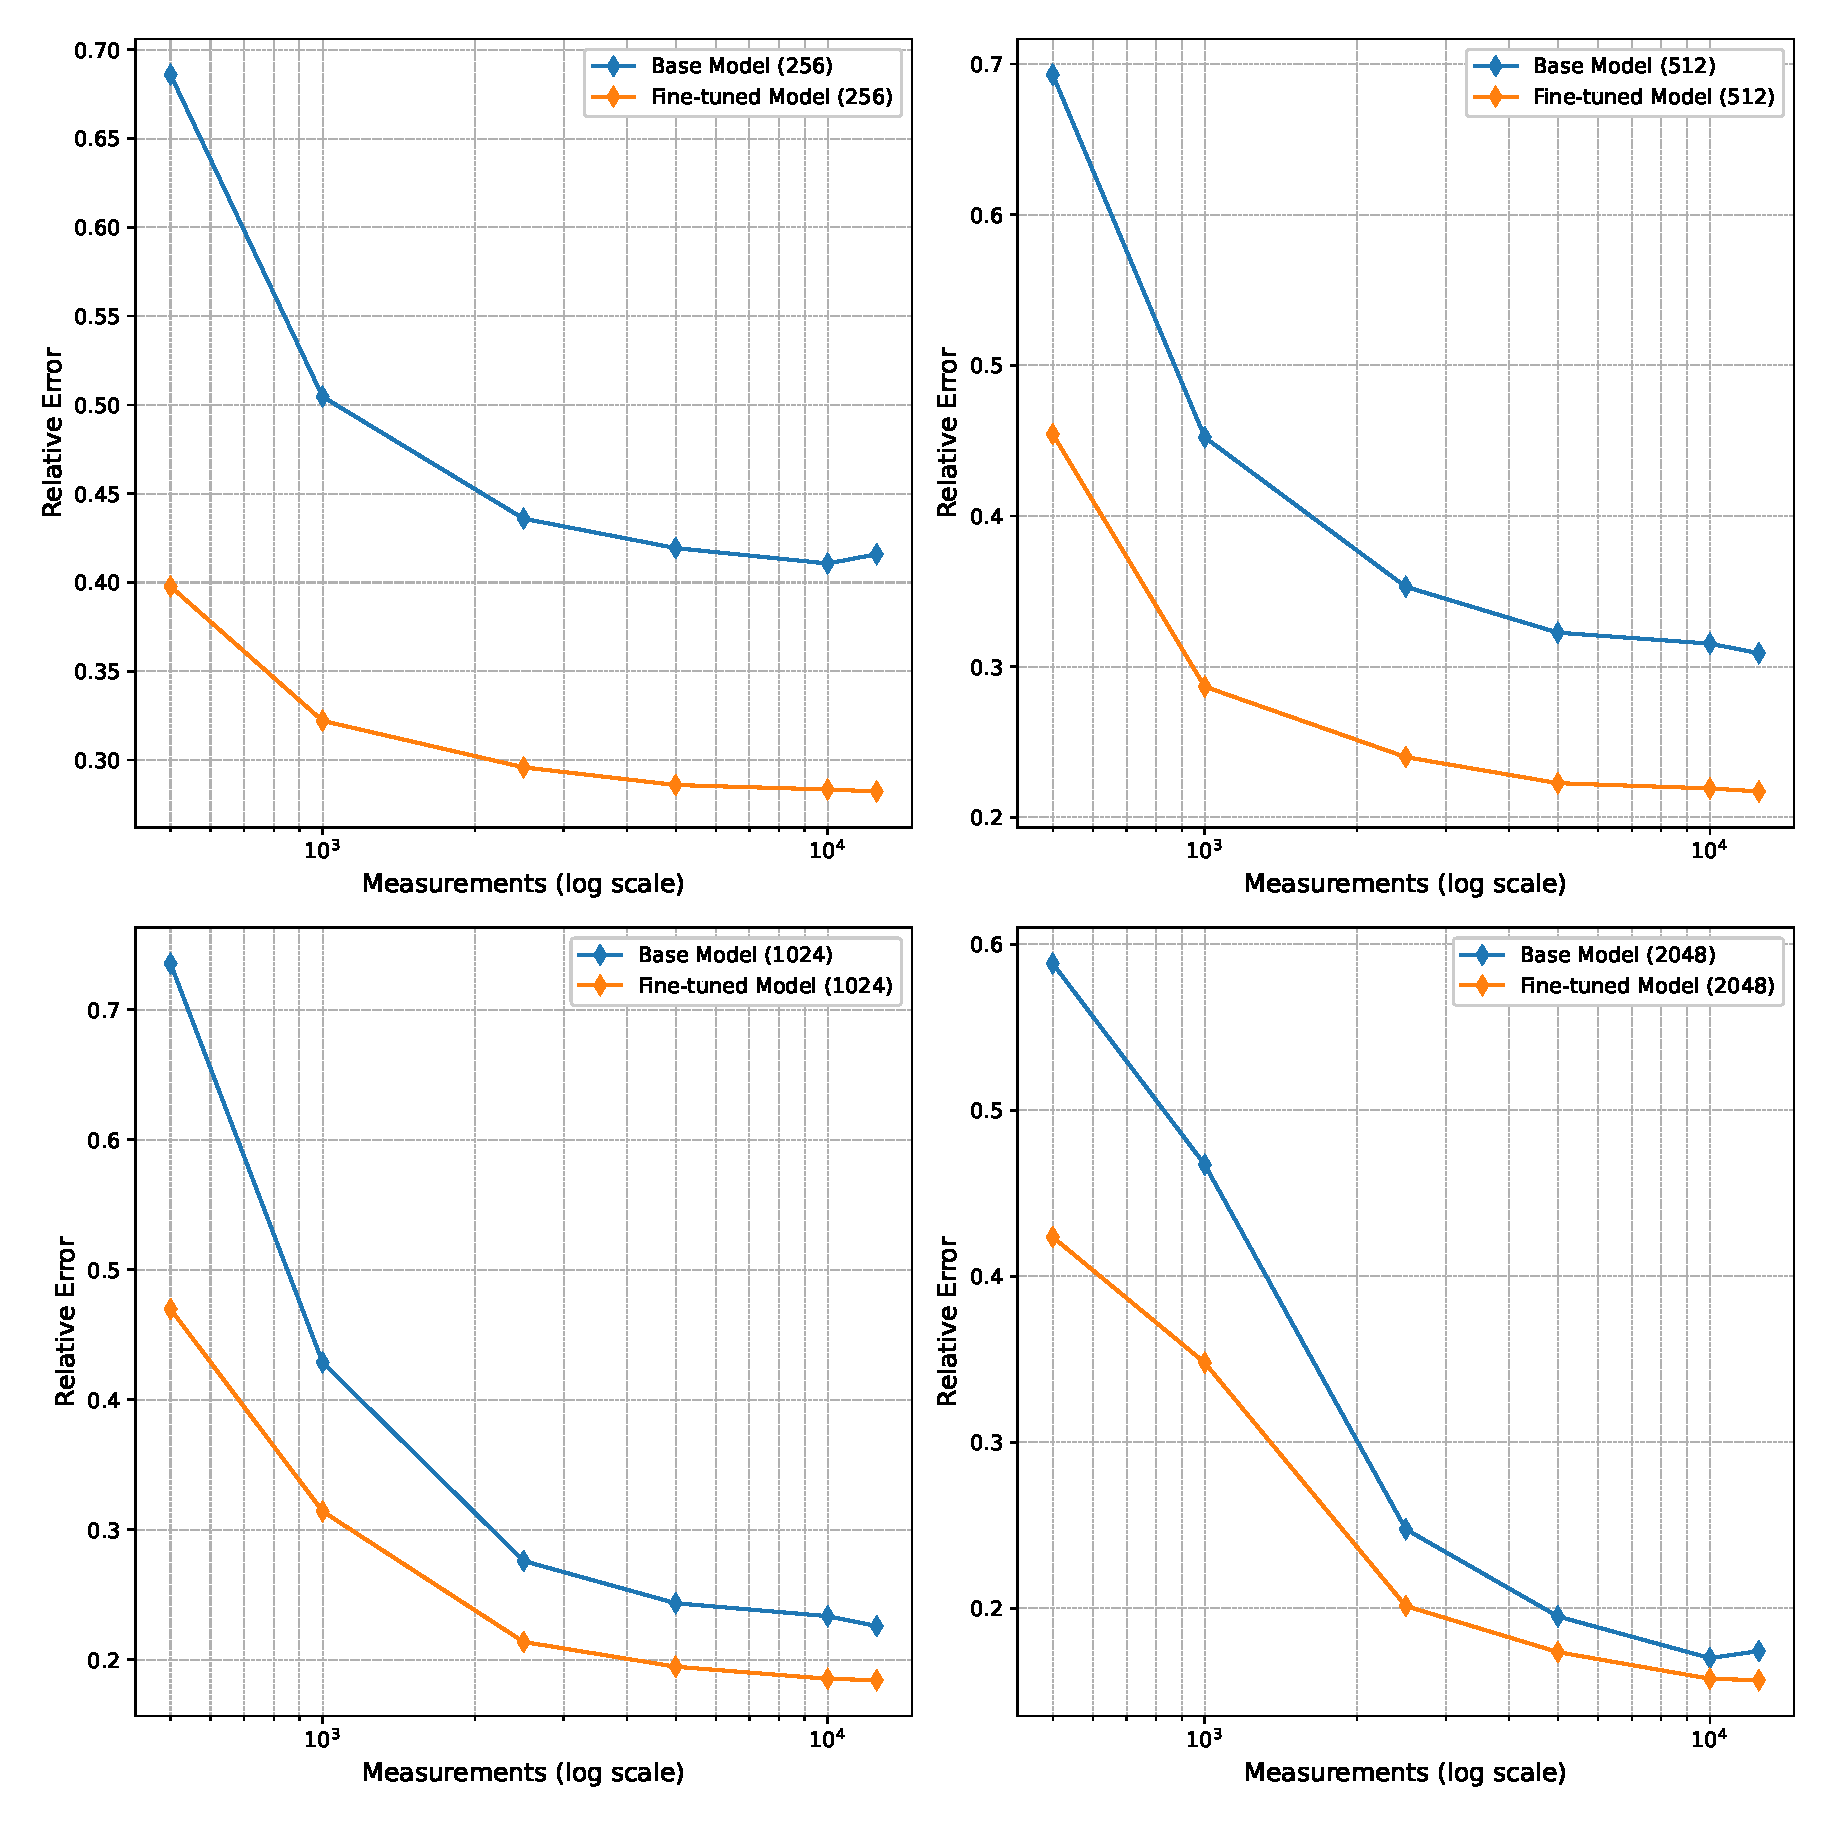
\includegraphics[width=\textwidth]{figures/06_results/fine_tuned_zuerich.eps}
    \caption{Results for Fine-tuned Model Zurich}
\end{figure}
The other plots can be seen in the appendix.
Overall, they follow the same trend.

\section{Generative Models vs Lasso}
\begin{figure}[h!]
    \centering
    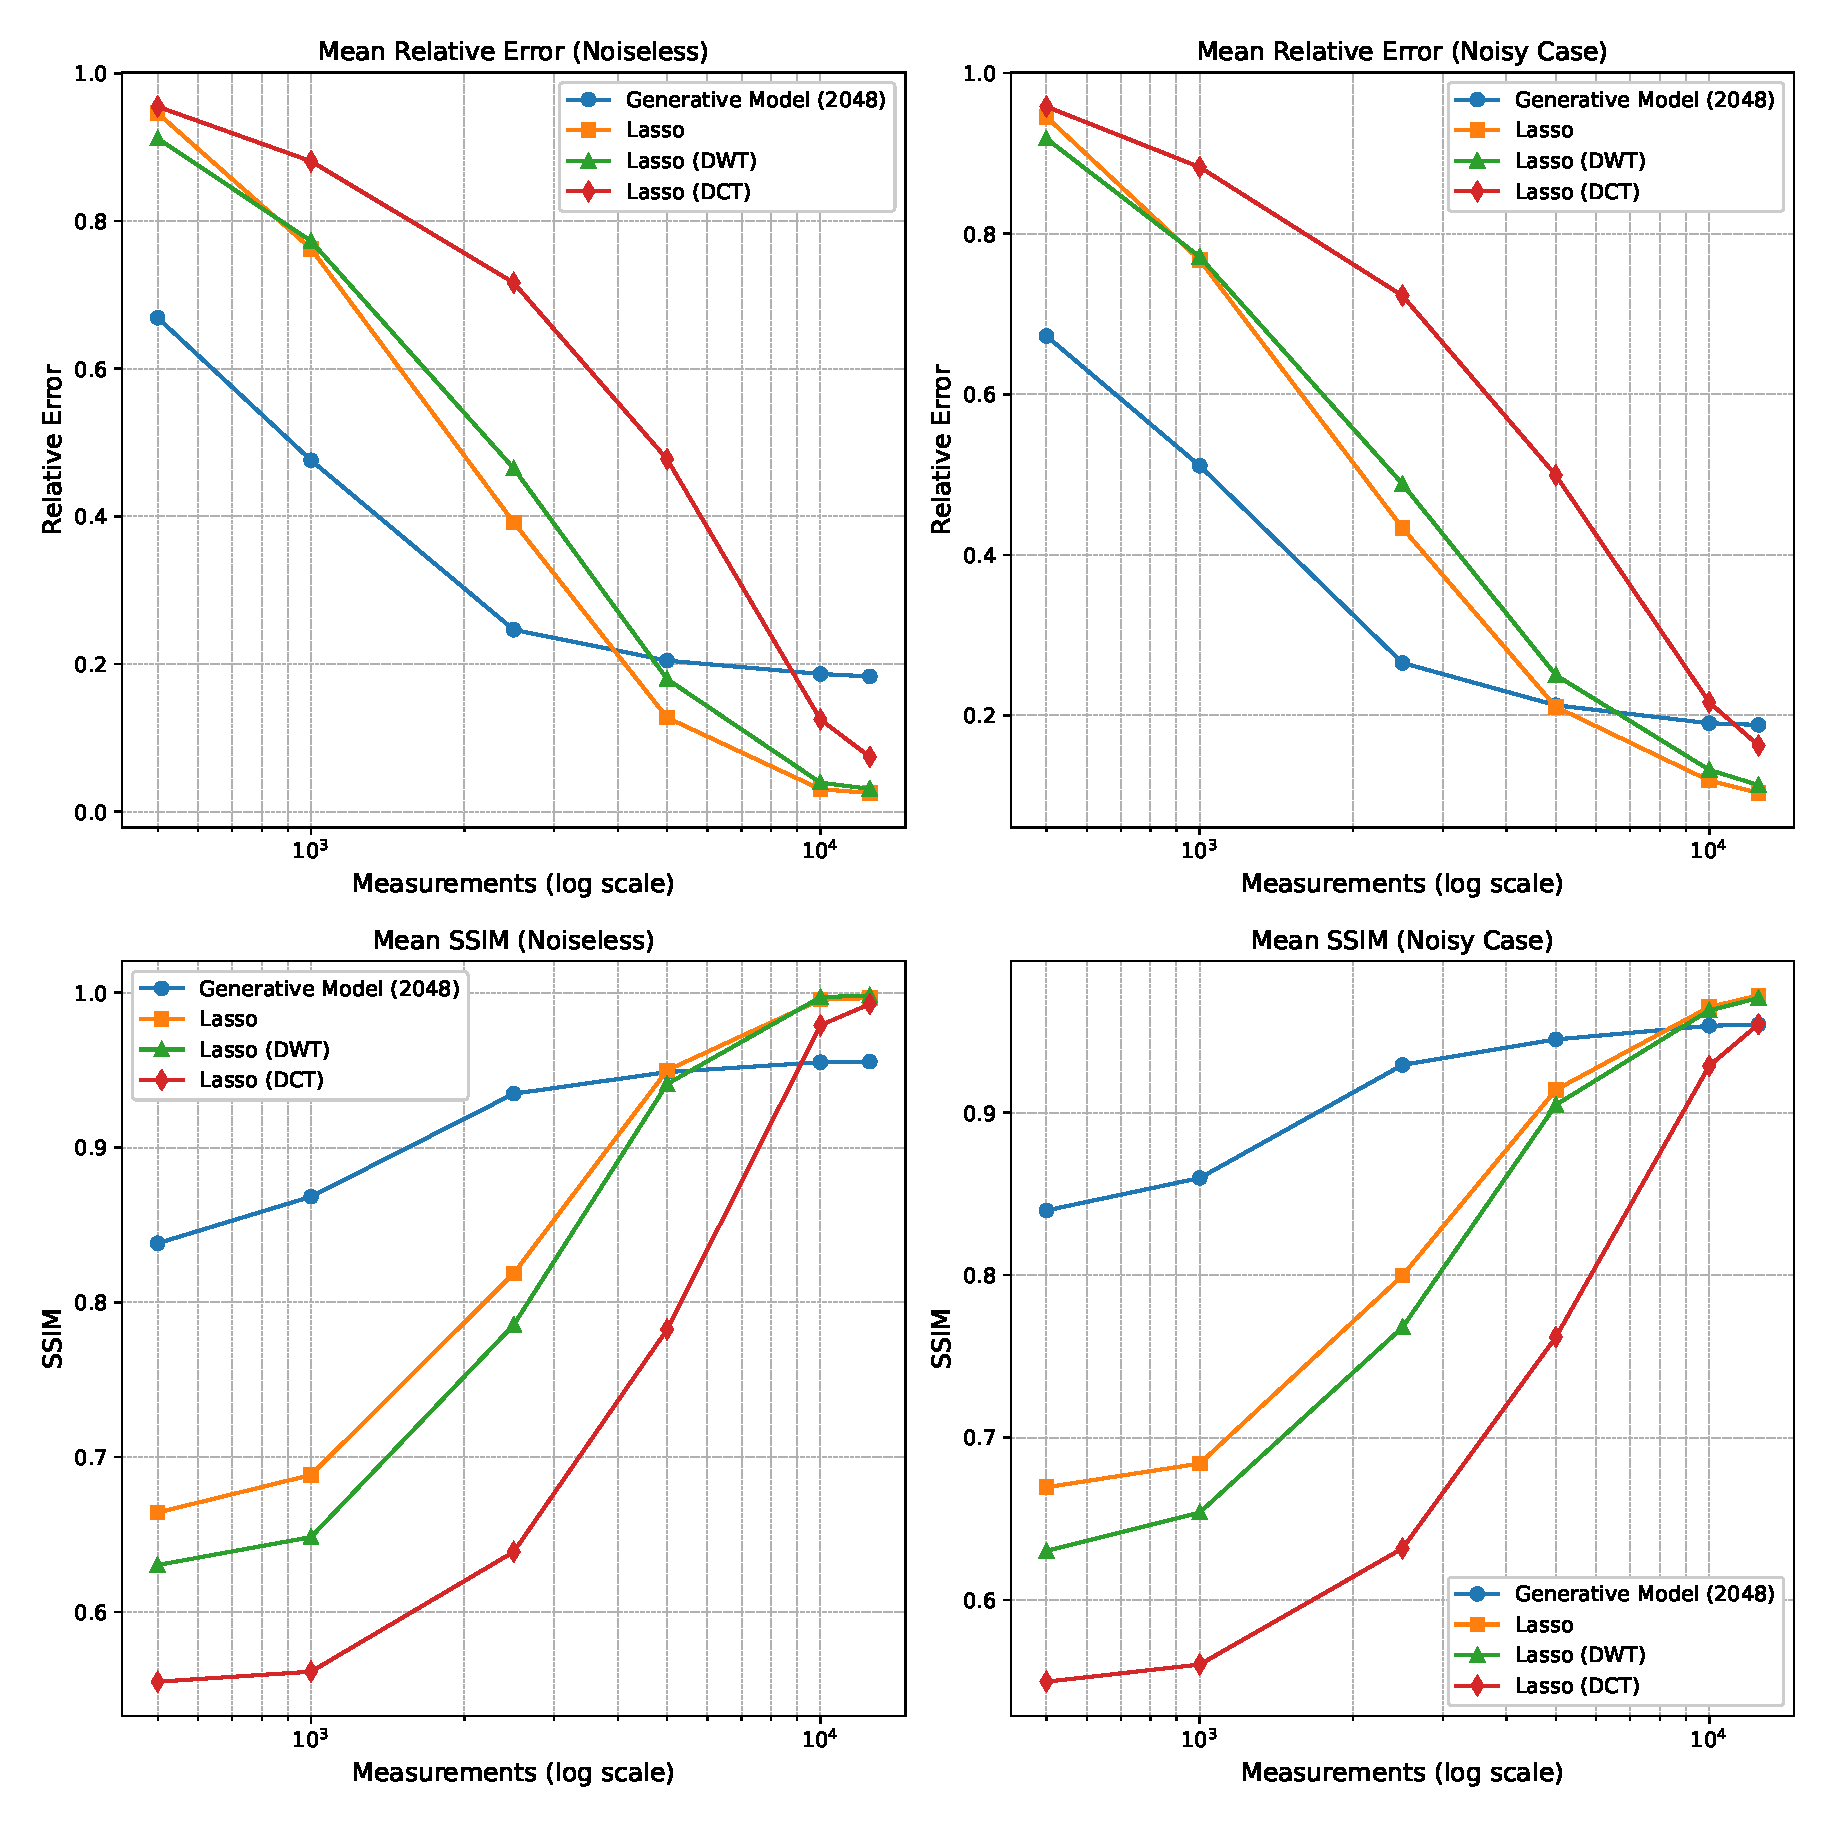
\includegraphics[width=\textwidth]{figures/06_results/gen_vs_lasso.eps}
    \caption{Generative Model vs Lasso}
\end{figure}
Make a graph that keeps num measurements fixed and only varies the noise.

\section{Gaussian Plume Model}
To fill.

Make a plot that has x axis snr and y axis relative error just like in Benjis plot.
Do this for the 3 cities.

Example Munich for low noise, i.e. 40db SNR.
\begin{figure}
    \centering
    \begin{subfigure}[b]{0.32\textwidth}
        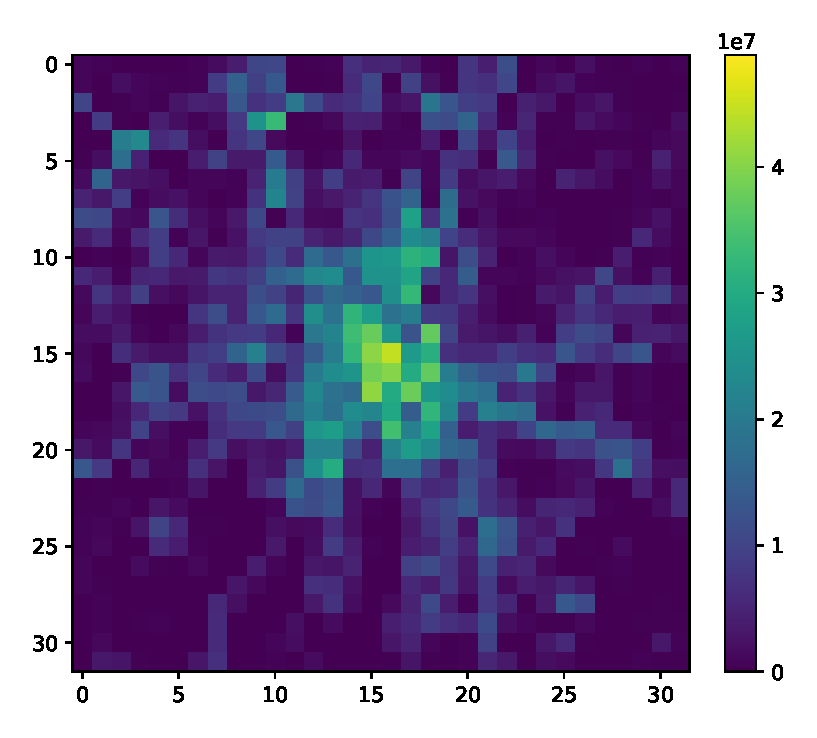
\includegraphics[width=\textwidth]{figures/06_results/gaussian_plume_example/munich/target.eps}
        \caption{Target Munich}
    \end{subfigure}
    \begin{subfigure}[b]{0.32\textwidth}
        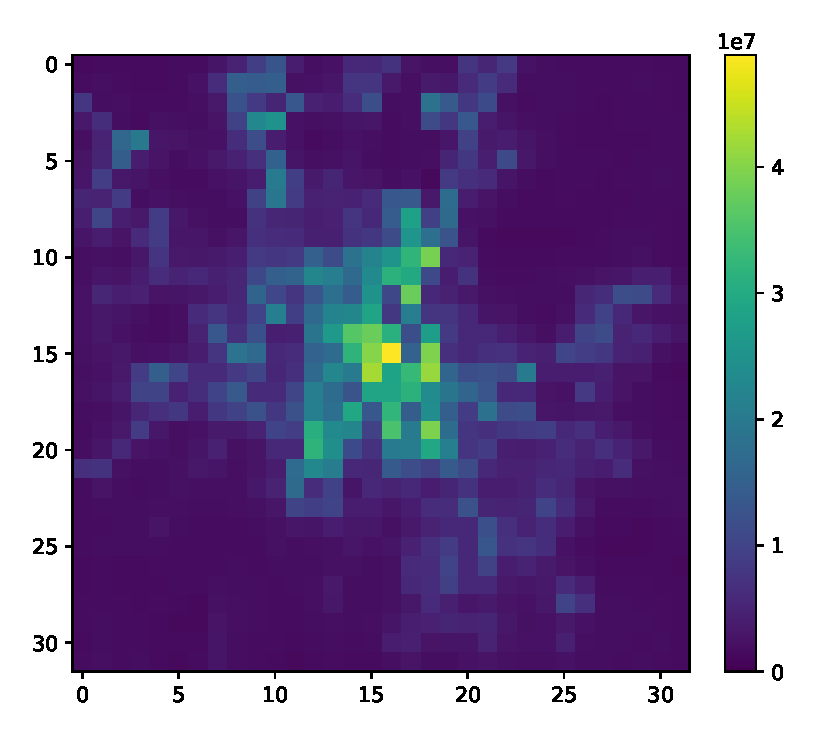
\includegraphics[width=\textwidth]{figures/06_results/gaussian_plume_example/munich/gen_2048_fine_tuned_40_db.eps}
        \caption{Gen 2048 Fine-tuned}
    \end{subfigure}
    \begin{subfigure}[b]{0.32\textwidth}
        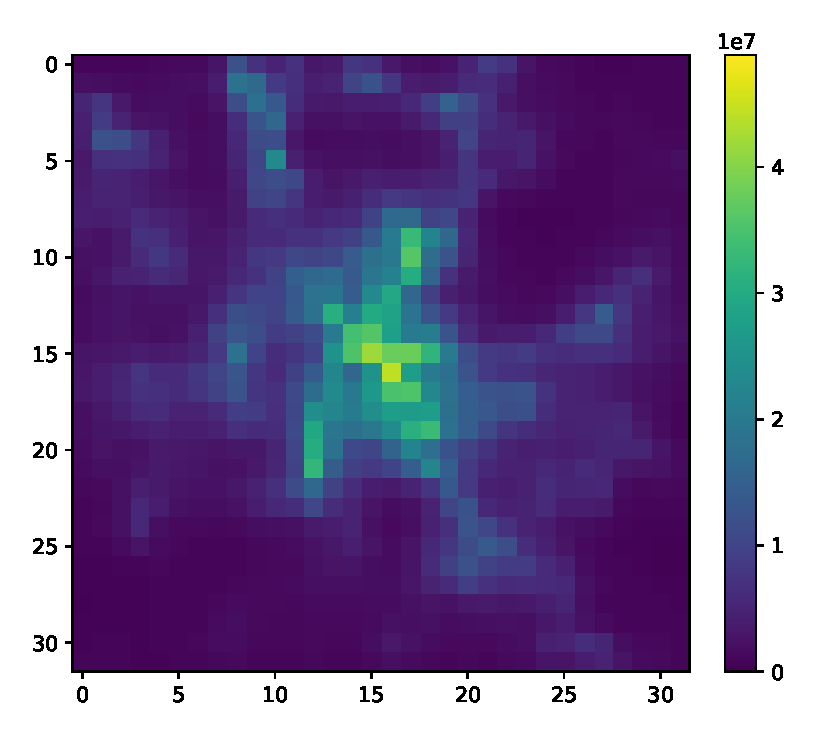
\includegraphics[width=\textwidth]{figures/06_results/gaussian_plume_example/munich/gen_2048_40_db.eps}
        \caption{Gen 2048}
    \end{subfigure}
    \begin{subfigure}[b]{0.32\textwidth}
        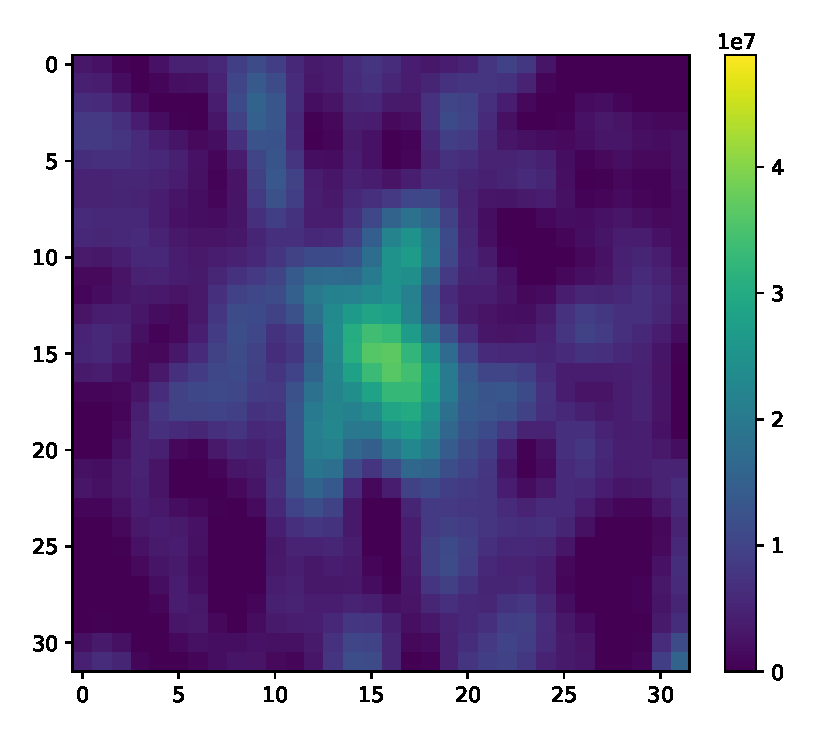
\includegraphics[width=\textwidth]{figures/06_results/gaussian_plume_example/munich/bp_dct_snr_40_db.eps}
        \caption{DCT}
    \end{subfigure}    
    \begin{subfigure}[b]{0.32\textwidth}
        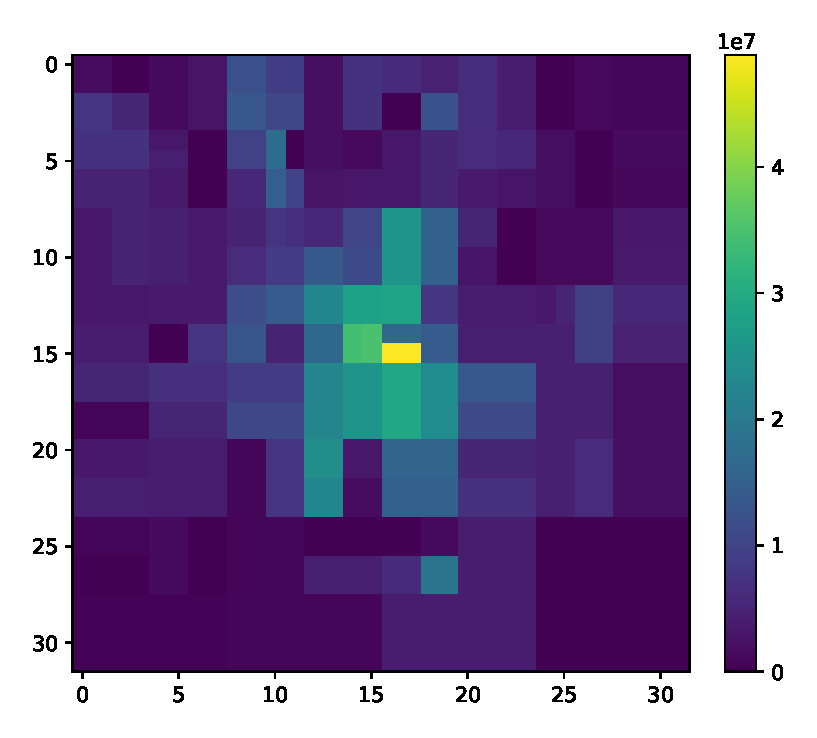
\includegraphics[width=\textwidth]{figures/06_results/gaussian_plume_example/munich/bp_dwt_snr_40_db.eps}
        \caption{DWT}
    \end{subfigure}
    \begin{subfigure}[b]{0.32\textwidth}
        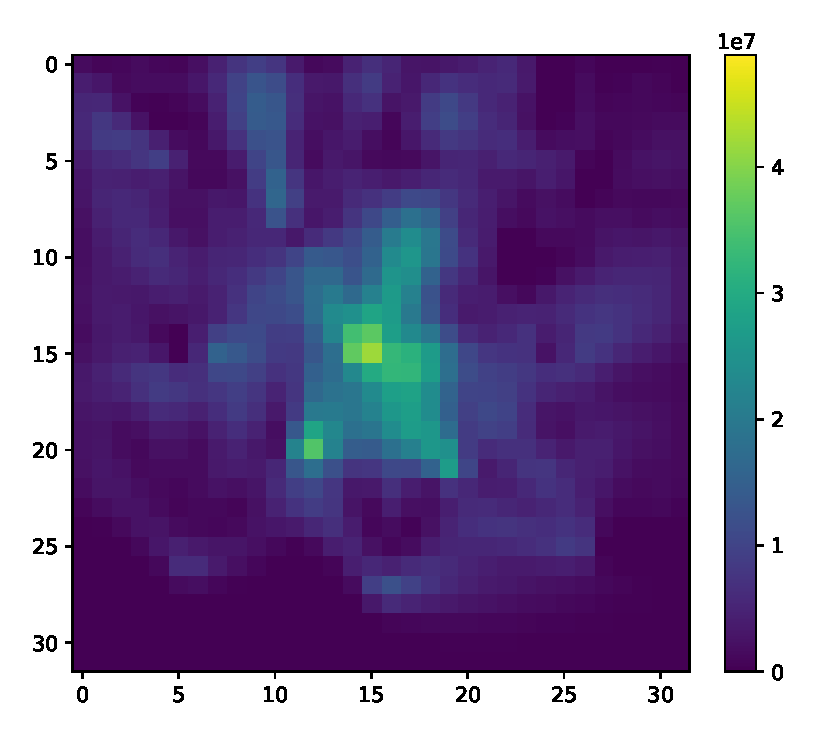
\includegraphics[width=\textwidth]{figures/06_results/gaussian_plume_example/munich/least_squares_snr_40_db.eps}
        \caption{LS}
    \end{subfigure}
    \caption{Target Munich}
\end{figure}

\section{Composition Into Sectors}


% !TeX root = ../main.tex
% Add the above to each chapter to make compiling the PDF easier in some editors.

\chapter{Discussion}\label{chapter:discussion}

\section{Discussion on Results}

\subsection{VAE Benchmark}

The experiments investigating the \gls{VAE}'s latent dimension provide insights into the trade-offs between model complexity and reconstruction performance.
Larger latent dimensions $d$ expand the range of the generator, directly impacting the model's representational error.
As $d$ increases, the model captures more complex structures in the emission fields, leading to a smaller representational error.
However, larger dimensions also make the optimization more challenging, which is particularly noticeable when the number of measurements is low. 
These results underscore the importance of the generator range.
Ideally, this range would be as small as possible while still effectively capturing the emission field distribution.

The comparison between the \gls{VAE} and \gls{Lasso} approaches highlights that, while the \gls{VAE} exhibits generative capabilities specific to emission fields, the representational error remains large.
This error requires a big latent dimension to be countered effectively.
However, even with $d = 2048$, the \gls{VAE} is significantly outperformed by \gls{Lasso} at high measurement counts.
This suggests that while the \gls{VAE} can approximate the distribution of emission fields, there is significant room for improvement.
The observation that fine-tuning enhances the \gls{VAE}'s performance further supports this finding, as a generalized model would better handle test samples without fine-tuning.

\subsection{Atmospheric Inversion}

The base \gls{VAE} models exhibit promising potential, showcasing competitive performance with \gls{BPDN} and \gls{LS} solvers for Munich and Zurich.
Through fine-tuning, the \gls{VAE}s demonstrate significant enhancements over \gls{BPDN} and \gls{LS} for these cities, underscoring the value of this process.
However, the results for Paris are different.
The base models perform worse than \gls{BPDN} with \gls{DCT} or \gls{DWT} and \gls{LS}.
Even with fine-tuning, the \gls{VAE} can only match the performance of \gls{BPDN} (\gls{DCT}) and \gls{LS}.
This suggests that the \gls{VAE}'s generative range does not adequately capture Paris's emissions, potentially due to significant differences between Paris and the training samples.

\section{Discussion on VAE}

The previous discussion reveals that the \gls{VAE} does not capture the emission field distribution perfectly.
High representational errors against \gls{Lasso} and the significant performance gains from fine-tuning illustrate this point.
The worse performance for Paris implies that specific emission patterns remain outside the \gls{VAE}’s generative range.

Further observations indicate that the trained models may not adequately map emission field space within the latent space.
The Gaussian-distributed latent variable $z$ can describe the prior emission fluxes.
Applying \gls{MCMC} \parencite{MCMC} algorithms with noisy observations can then solve the inverse problem as outlined in \cite{VAE-MCMC}.
However, \gls{MCMC} failed to converge for many samples, such as Munich, whereas it worked well for randomly generated samples from Gaussian-distributed $z$ values.
This suggests that the \gls{VAE}’s generator does not capture these samples fully.
Lastly, the observation that no regularization term $\gamma$ produced optimal results suggests that latent variables corresponding to test samples lie far from the center, thus indicating that the \gls{VAE} does not capture these samples well.

Overall, from these five observations, it can be argued that the trained \gls{VAE} failed to capture the emission field distribution fully.

The key contributing factor to this limitation is likely the need for more diverse training samples.
With $74$ unique cities in the training data, the information a machine learning model can extract is limited.
It can be expected that with more unique training samples, the generalization capabilities of the \gls{VAE} improve \parencite{limited-data}, thus capturing the emission field distribution better.

\section{Challenges}
Besides the limitations regarding the \gls{VAE}, two further challenges of the presented method need to be discussed.
The first challenge is the validation of the inverse models.
The second challenge is the quantification of uncertainties in the inverse model outputs.

\subsection{Validation of Inverse Model}
A fundamental issue within this thesis is that the ground truth relies on emission inventories, which may contain inaccuracies due to various factors.
This makes real-world validation challenging.
Similarly, real-world measurements complicate validation since the ground truth is often unknown.
A potential solution could involve controlled release experiments, where emissions are measured and quantified in a controlled environment to validate inversion methods.
However, such experiments come with their challenges, mainly due to the resolution of the model and the scale of emission fluxes.
Therefore, validation of the presented inverse model remains an open research field.

\subsection{Uncertainty Quantification}

The inverse models presented in this thesis, i.e., sparse reconstruction, \gls{LS}, and the \gls{VAE}, cannot quantify uncertainties in the reconstructed outputs.
In particular, the \gls{VAE} approach presented in this thesis outputs an estimation of the \gls{MAP} but does not quantify the certainty of this estimation.
However, extending the presented inverse model with uncertainty quantification is possible.
Specifically, as outlined before, \gls{MCMC} \parencite{MCMC, VAE-MCMC} can be applied to sample from the posterior distribution of the predictions.
This enables the computation of both the mean and variance, where the variance provides a measure of uncertainty in the predictions.
That said, as initial attempts with \gls{MCMC} showed convergence issues for certain test samples, it is essential to first address the limitations in training sample diversity to ensure the robustness of the model’s posterior distribution before applying \gls{MCMC} for reliable uncertainty quantification.

\section{Deviation from Inventories}

The experiments and benchmarks demonstrate that fine-tuning significantly improves the relative error and \gls{SSIM} of reconstructions using the \gls{VAE}s.
However, an important consideration regarding the evaluation methodology needs to be addressed.
The models undergo fine-tuning using $2015$ inventory data with data augmentation using noise and various scaling factors, while testing is conducted on $2018$ data.
Given the substantial similarity between the $2015$ and $2018$ datasets, the enhanced performance on reconstruction tasks is expected.
However, this evaluation inherently assumes that the $2018$ inventory represents the ground truth.

The critical question that remains unanswered is how these models perform when the actual ground truth deviates from the inventory data.
This consideration is particularly relevant for fine-tuned models, where the assumed ground truth closely resembles the training data, unlike base models where test data differs significantly from training samples.

Consequently, future work should extend the evaluation framework to assess the fine-tuned models' capability to reconstruct deviations from the actual inventories.
For instance, further experiments could involve artificially injecting emission sources and evaluating the models' ability to accurately reconstruct these injected emitters.
Such an approach would provide more robust insights into the models' true reconstruction capabilities when confronted with emission patterns that deviate from the training inventory data.

\section{Future Applications}
Despite the limitations and challenges outlined, several positive takeaways from the results can be leveraged for future work.

Firstly, the base \gls{VAE} models have shown they can match the performance of traditional methods like \gls{LS} and sparse reconstruction techniques and, in certain low-noise cases, even outperform them.
The fine-tuned models demonstrate even more promising results, significantly improving upon the base models and outperforming conventional approaches for Munich and Zurich.
This is particularly notable given the limited training data, suggesting that \gls{VAE}s and similar machine-learning models have strong potential in atmospheric inversion tasks.

From these observations, we can extrapolate that machine-learning models may play a crucial role in the future of atmospheric inversion.
Addressing the primary issue of limited data is essential for realizing this potential.
By scaling up the training data and including more diverse and unique samples, the generalization capabilities of machine learning models are expected to improve significantly, as suggested by \parencite{limited-data}. This would enable the models to better capture the distribution of emission fields and reduce representational errors.

Furthermore, exploring different model architectures could help overcome current limitations.
For example, training models like normalizing flows \parencite{NormalizingFlows} with no representational error could be highly beneficial.
These models can capture the emission field distribution more accurately, leading to improved inversion results.

In particular, many inspirations can be taken from different fields of research, such as medical imaging, where state-of-the-art inversion approaches rely heavily on machine learning models \parencite{ReviewCSUsingAI}.
Techniques like score-based models \parencite{ScoreBased}, which have shown remarkable results in other domains, could be adapted and applied to atmospheric inversion.
By integrating these advanced methods, it is possible to develop more accurate and robust inversion techniques.
Overall, the findings of this thesis open new possibilities for future research.

\section{Research Questions}
This section revisits the research questions outlined at the start of this thesis and discusses whether these questions have been addressed through the experiments and analyses performed.
\\\\
\textbf{To what extent can a \gls{VAE} capture meaningful low-dimensional representations of area-source emissions in urban inventories?}
\\
The evaluation of this question is based on the benchmark inspired by the work of Bora et al., as detailed in Section \ref{section:vae_benchmark}.
Experimental results indicate that \gls{VAE}s can capture a low-dimensional representation of emission fields.
For instance, the \gls{VAE} with a latent dimension of $d=2048$ achieved an average reconstruction with a \gls{SSIM} of approximately $0.95$ and a relative error of around $20\%$.
This corresponds to a dimensionality reduction of approximately $86.7\%$, showing that meaningful latent variables corresponding to test samples can be identified.
These findings support the argument that the trained \gls{VAE}s successfully capture a low-dimensional representation of area-source emissions.
\\\\
\textbf{How does the choice of latent space dimensionality in the \gls{VAE} impact the quality and accuracy of emission reconstructions?}
\\
To answer this question, the benchmark in Section \ref{section:vae_benchmark} can be utilized, mainly focusing on experiments where the latent dimension $d$ varied across the values $\{ 256, 512, 1024, 2048 \}$.
Results suggest a trade-off between the latent dimensionality and reconstruction performance.
A higher latent dimension $d$ enhances representational complexity, thus reducing the representational error.
However, a larger dimension makes it more challenging to efficiently search through the representation space, especially with lower measurement counts.
In these cases, models with smaller latent dimensions performed better regarding \gls{SSIM} and relative error.
This suggests an optimal target of minimizing the representational error while keeping $d$ as low as possible.
\\\\
\textbf{To what extent is the \gls{VAE} generalizable across diverse urban emission fields, or does it benefit from fine-tuning for specific cities?}
\\
This question can be answered by analyzing the results from Subsection \ref{subsection:latent_dimension} and Section \ref{section:atmospheric_inversion_results}.
While the base models demonstrate a strong performance across various urban fields, fine-tuning significantly improves their relative error and \gls{SSIM}.
This improvement is particularly evident in atmospheric inversion, where measurements are highly correlated and sparse. \gls{VAE}s show promising generalizability, but fine-tuning yields substantially better performance, especially in data-limited contexts.
\\\\
\textbf{How well does such a variational autoencoder perform in atmospheric inversion of area sources as a downstream task compared to state of the art approaches?}
\\
The results presented in Section \ref{section:atmospheric_inversion_results} indicate that baseline \gls{VAE} models perform competitively in atmospheric inversion tasks, particularly excelling in \gls{SSIM} metrics, as demonstrated by the results for Munich.
For Paris, the reconstructions of the baseline \gls{VAE} fall behind the classical solvers as the emission flux field of Paris does not seem to be adequately represented in the generator range.
However, with fine-tuning, \gls{VAE}s significantly outperform the classical solvers for Munich and Zurich, and reach comparable performance for Paris.
The more detailed case study for Munich shows that, at a moderate to high \gls{SNR} of $20 \unit{dB}$, the baseline \gls{VAE} achieves higher \gls{SSIM} and lower relative error than the other classical solvers.
The fine-tuned model outperforms other methods at a reduced \gls{SNR} of $5 \unit{dB}$, while the baseline \gls{VAE} fails to deliver adequate reconstructions.

% !TeX root = ../main.tex
% Add the above to each chapter to make compiling the PDF easier in some editors.

\chapter{Conclusion and Future Work}\label{chapter:conclusion}

\section{Paradigm Shift}
This work can be seen as paradigm shift in inversion approaches for atmospheric inversion.


\appendix{}
% \input{chapters/09_appendix}

\microtypesetup{protrusion=false}

%\addchap{Abbreviations}
%\begin{acronym}
%\itemsep-.25\baselineskip
%\acro{TUM}[TUM]{Technical University of Munich}
% TODO: add acronyms
%\end{acronym}

\listoffigures{}
\listoftables{}
\microtypesetup{protrusion=true}
\printbibliography{}

\end{document}
